\nonstopmode
\documentclass[10pt, a4paper]{article}
%\usepackage{subfig}

\parindent=20pt
\parskip=8pt
\usepackage[width=15.5cm, left=3cm, top=2.5cm, height= 24.5cm]{geometry}
\usepackage[spanish]{babel}
\usepackage[utf8]{inputenc}
\usepackage{fancyhdr}
\usepackage{multirow}
\usepackage{rotating}
\usepackage{indentfirst}
\usepackage{latexsym}
\usepackage{caratula}
\usepackage{gnuplottex}
\usepackage{epsfig}
\usepackage{lastpage}
\usepackage{amsfonts}
\usepackage{listings}
\usepackage[export]{adjustbox}
\usepackage{pdfpages}
\lstset{language=C}
\usepackage[ruled,vlined,linesnumbered]{algorithm2e}
\usepackage{graphicx}
\usepackage{float}
\usepackage{color}

\graphicspath{{imgs/}}



% Acomodo fancyhdr.
\pagestyle{fancy}
\thispagestyle{fancy}
\addtolength{\headheight}{1pt}
\lhead{Algoritmos y Estructuras de Datos III}
\rhead{TP3}
\cfoot{\thepage /\pageref{LastPage}}
\renewcommand{\footrulewidth}{0.4pt}
\renewcommand{\thesubsubsection}{\thesubsection.\alph{subsubsection}}


\author{Algoritmos y Estructuras de Datos III, DC, UBA.}
\date{}
\title{}

\begin{document}
	
\thispagestyle{empty}
\materia{Algoritmos y Estructuras de Datos III}
\submateria{Trabajo Pr\'actico N$^{\circ}$3}
\titulo{}
\integrante{Izcovich, Sabrina}{550/11}{sizcovich@gmail.com}
\integrante{Garcia Marset, Matias}{356/11}{matiasgarciamarset@gmail.com}
\integrante{Orellana, Ignacio}{229/11}{nacho@foxdev.com.ar}
\integrante{Vita, Sebastián}{149/11}{sebastian\_vita@yahoo.com.ar}

\maketitle

\tableofcontents
\newpage

\section{Introducci\'on}
El siguiente trabajo práctico consiste en un estudio de distintas formas de resolver un mismo problema algorítmico a partir de diversas técnicas.

El problema se basa en hallar la clique\footnote{Dado un grafo simple $G$ = ($V;E$), un subconjunto de vértices de $G$ es una clique sí y sólo sí éste induce un subgrafo completo de $G$.} de máxima frontera\footnote{Definimos la frontera de una clique como $\delta(K) = \left \{ vw \in E / v \in K \land w \in V \setminus K \right \}$.} (CMF) de un grafo. Es decir que, dado un grafo $G$, debemos encontrar una clique $K$ cuya frontera $\delta(K)$ tenga cardinalidad máxima. Para resolver el problema, supondremos que los grafos son simples, con lo cual no tienen bucles ni ejes repetidos.


\textbf{Formato de entrada:}
La entrada contiene varias instancias del problema. Cada instancia representa un grafo $G$ y comienza con una línea con dos valores enteros $n$ (cantidad de vértices) y $m$ (cantidad de aristas). A continuación, le siguen $m$ líneas, cada una determinando una arista del grafo, cuyo formato es el siguiente:
$$v_{1}\ v_{2}$$
donde $v_{1}$ y $v_{2}$ son los extremos de la arista representada (numerados de 1 a $n$).

\textbf{Formato de salida:} 
La salida contiene una línea por cada instancia de entrada, con el siguiente formato:
$$F\ k\ v_{1}\ v_{2}\ ...\ v_{k}$$
donde $F$ es el cardinal de la frontera de la clique dada como solución, $k$ es el tamaño de la misma y $v_{1}$, ..., $v_{k}$ son los vértices que la conforman.\newline


Para resolver el problema presentado, debimos diseñar e implementar los siguientes tipos de algoritmos:

\begin{itemize}
 \item Un algoritmo exacto.
 \item Al menos una heurística constructiva golosa.
 \item Al menos una heurística de búsqueda local.
 \item Al menos un algoritmo que use la metaheurística \textit{Búsqueda Tabú}\footnote{Fred Glover. Tabu Search - Part 1. ORSA Journal on Computing 1 (3), pp: 190 \& Part 2. ORSA Journal on Computing 2 (1), pp: 4.}
\end{itemize}

El trabajo se organizó de la siguiente forma:
\begin{itemize}
\item El \textbf{ejercicio 1} fue utilizado para describir situaciones de la vida real que pudieran ser modeladas utilizando CMF.
\item En el \textbf{ejercicio 2}, diseñamos un algoritmo exacto para CMF explicando detalladamente su implementación. Luego, calculamos el orden de complejidad temporal del peor caso. Finalmente, explicitamos la experimentación realizada capaz de comprobar la performance del algoritmo realizado comparando su tiempo de ejecución en función del tamaño del parámetro de entrada.
\item El \textbf{ejercicio 3} consistió en presentar distintos tipos de heurísticas, constructivas golosas y de búsqueda local, que resolvieran el problema descrito como también algoritmos que utilizaran la metaheurística Búsqueda Tabú. Cada algoritmo debió ser explicado detalladamente y su orden de complejidad temporal debió ser explicitado al igual que instancias de CMF para las cuales los métodos no proporcionan una solución óptima. Por último, se realizó la experimentación necesaria para observar la performance de cada algoritmo comparando la calidad de las soluciones obtenidas y los tiempos de ejecución de los mismos en función de la entrada.
\item Finalmente, en el \textbf{ejercicio 4}, evaluamos los algoritmos propuestos sobre un nuevo conjunto de instancias una vez elegidos los mejores valores de configuración para cada heurística.
\newpage

\section{Descripción de situaciones reales}
En este ejercicio, nos limitamos a pensar situaciones de la vida real que pudieran ser modeladas con $cliques\ de\ máxima\ frontera$.
\begin{itemize}

\item La conocida empresa internacional \textit{Chumbawamba} decide formar un equipo de trabajo para un proyecto que cambiará el mundo. Para que éste funcione sin peleas de por medio, dicho equipo debe consistir en un grupo de personas que se conozcan entre sí. Dado que la empresa desea que el proyecto sea conocido por la mayor cantidad de gente posible (siendo el boca en boca su única forma de difusión), deciden seleccionar a sus empleados de acuerdo a un conjunto que se conozca entre sí y que, también, conozca a la mayor cantidad de gente posible fuera de la empresa. Para modelar este problema, se consideran a los nodos como personas y a las aristas como la representación de un vínculo existente entre una persona y otra.

\item Un conocido golpeador desea asistir a la mejor fiesta todos los tiempos. Debido a su tardío horario de llegada al evento, éste se percata de que no puede bailar tranquilamente en el espacio reducido que encontró. Bajo un ataque de furia decide comenzar a pegarle a la gente de forma estratégica para que, al tirar a una persona, se produzca un efecto dominó y se caigan todas las que se encuentran a menos de treinta centímetros de ésta. De este modo, lograría tirar la mayor cantidad de gente al piso y disfrutar de la fiesta tranquilo. Luego, nota que le conviene comenzar a golpear a las personas que se encuentran a menos de un metro y medio de distancia entre sí y que, además, se encuentran a menos de dicha distancia con la mayor cantidad de personas para que el alcance sea mayor. Para modelar este problema, consideramos a los nodos como personas y a las arista como la representación de que la distancia entre una persona y otra es menor a un metro y medio.  

\item En un campo casi como cualquier otro, se encuentran plantas que deben ser regadas con gran potencia para no morir. Debido a que, a medida que el agua atraviesa una planta, ésta pierde potencia, el granjero \textit{Don Omar} busca que la mayor cantidad de plantas sean regadas con la mayor potencia posible. Dado que el granjero es una persona de gran capacidad pero no posee un enorme presupuesto, decide armar una estrategia de riego para sus amadas plantas teniendo que seleccionar un único circuito. Como cuenta con un único circuito de riego en el que Ésta consiste en regar alguna planta dentro de un cí de para que se muera la menor cantidad de plantas. Para modelar este problema, se consideran a los nodos como plantas y a las aristas como caminos del sistema de riego por donde puede circular el agua. %no esta terminado

\item Juanita es una apasionada de conocer calles nuevas y desea mudarse a una ciudad que le permita seguir con su pasión. Pero Juanita trabaja en el campo, o sea que fuera de cualquier ciudad, así que se le ocurre seleccionar su próxima vivienda de acuerdo a la cantidad de calles que va a poder conocer para llegar al campo. Podemos modelar el problema como los nodos representantes de las esquinas y las aristas las interconexiones entre éstas. Llamamos ciudad a todas las esquinas que se conectan todas con todas, luego, a una clique y campo a todo lo que se encuentra entre una ciudad y otra. Por lo tanto, se desea encontrar una ciudad con mayor frontera para que la cantidad de posibles calles nuevas a recorrer fuera de la ciudad sea la mayor.

\end{itemize}

\newpage

\section{Detalles de implementación}
Para la realización de las Heurísticas Golosa, Búsqueda Local y Búsqueda Tabú, utilizamos la clase \textit{Grafo}. Dicha clase fue establecida a partir del Taller de Heurísticas\footnote{http://www.dc.uba.ar/materias/aed3/2013/2c/laboratorio/taller-heuristicas/view} realizado en los laboratorios. En ella, se hace uso de un vector de adyacencia y una matriz de adyacencia, dependiendo del caso. Por ejemplo, para saber si dos nodos son vecinos, resulta más simple utilizar una matriz de adyacencia pues simplemente debe verificarse una única posición. Por otro lado, para obtener la totalidad de los vecinos de un nodo, es conveniente usar un vector de adyacencia pues no es necesario recorrer ninguna estructura para obtener dicho resultado. 

Analicemos la complejidad temporal de la clase \textit{Grafo}:
\begin{itemize}
\item \textbf{Definición de grafo:}
\begin{itemize}
\item $vecinos(nodos, vuint()) \rightarrow \mathcal{O}(n)$ pues $vecinos$ es $std::vector< vuint > vecinos$ y por cada elemento debe realizarse un $push\_back$($\mathcal{O}(1)$ amortizado)\footnote{http://www.cplusplus.com/reference/vector/vector/push\_back/}, siendo $\mathcal{O}(n)*\mathcal{O}(1) = \mathcal{O}(n)$ el resultado final.
\item $adyacencia(nodos, std::vector<bool>(nodos, false)) \rightarrow \mathcal{O}(n^2)$ pues $adyacencia$ es $std::vector<std::vector<bool> > adyacencia$ y realiza $n\ push\_back$ por cada elemento, luego, su complejidad temporal resulta $\mathcal{O}(n)*\mathcal{O}(1)*\mathcal{O}(n)*\mathcal{O}(1) = \mathcal{O}(n^2)$.
\item $cnodos(nodos) \rightarrow \mathcal{O}(1)$ pues $nodos$ es $uint\ cnodos$.
\end{itemize}
\item \textbf{Funciones públicas:}
\begin{itemize}
\item $nodos$ devuelve $cnodos$, luego su complejidad es $\mathcal{O}(1)$.
\item $sonVecinos$ accede a una posición de $adyacencia$, luego, su complejidad temporal es $\mathcal{O}(1)*\mathcal{O}(1) = \mathcal{O}(1)$\footnote{http://www.cplusplus.com/reference/vector/vector/operator[]/}.
\item $agregarArista$ realiza dos $push\_back (\mathcal{O}(1) + \mathcal{O}(1) = \mathcal{O}(1)$) al vector $vecinos$ y, finalmente, le asigna un valor booleano a dos posiciones de $adyacencia$, siendo esto $\mathcal{O}(1)$ amortizado\footnote{http://www.cplusplus.com/reference/vector/vector/assign/}.
\item $vecindad$ retorna el valor de un elemento del vector $vecinos$, luego, la complejidad resulta $\mathcal{O}(1)$\footnote{http://www.cplusplus.com/reference/vector/vector/operator[]/}.
\item $nodoDeMayorGrado$ recorre la totalidad de los nodos ($cnodos$) del grafo (en $\mathcal{O}(n)$). En cada iteración, compara el tamaño (utilizando la función size() ($\mathcal{O}(1)$)\footnote{http://www.cplusplus.com/reference/vector/vector/size/}) de los vecinos de dos nodos y asigna un valor a un uint ($\mathcal{O}(1)$) dependiendo del resultado de la comparación. Luego, la complejidad temporal de dicha función resulta $\mathcal{O}(n)$.
\item $frontera$ recorre los nodos de una clique del grafo (cuyo tamaño máximo es $n$) y le asigna a un $uint$ el tamaño (utilizando size()) de un acceso a $vecinos$ ($\mathcal{O}(1)$). Luego, la complejidad de la función resulta $\mathcal{O}(n)*\mathcal{O}(1) = \mathcal{O}(n)$.
\end{itemize}
\end{itemize}

\newpage
\section{Algoritmo Exacto}
\subsection{Explicación del algoritmo realizado}

Para resolver el problema de CMF de forma exacta, generamos un algoritmo encargado de recorrer todas las posibles cliques del grafo de entrada con la estrategia de $Backtracking$. Esto se debe a que no hallamos ninguna caracterización particular que nos permitiera reducir el espacio de búsqueda de cliques tal que el algoritmo ignorara una cantidad asintótica de ellas. Luego, nuestra implementación genera todas las soluciones posibles siguiendo un orden lexicográfico para evitar repetirlas. Por ejemplo, la clique $k_{2}$ formada por los nodos \{1,2\} es la misma que se forma al elegir los nodos \{2,1\}. Por lo tanto, al representar los nodos como números y formar cliques respetando su orden lexicográfico, nos ahorramos realizar repeticiones como la mencionada. 

De este modo, nuestro algoritmo comienza generando todas las cliques que contienen al nodo de menor valor numérico que no haya sido utilizado y, en cada paso, selecciona una serie de candidatos a ser agregados a la clique actual hasta que no quede ninguno. Una vez alcanzada dicha instancia, el algoritmo retrocede quitando el último nodo agregado a la clique e insertando al próximo candidato, si es que existe. El orden lexicográfico se respeta al momento de elegir los candidatos ya que sólo pueden ser seleccionados como tales aquellos cuyo valor representativo sea mayor al del último nodo agregado a la clique.

A continuación, se expone el pseudocódigo del algoritmo mencionado:\\

\underline{Variables globales:} \textbf{Conj(nodo)} $cliqueMaxima$, \textbf{Entero} $fronteraMaxima$.\\

\begin{algorithm}[H]
	\SetAlgoLined
	\caption{Algoritmo Exacto}
	\KwIn{\textbf{Grafo} $g$}
	\KwOut{\textbf{Conj(nodo)} $clique$}

	\For{nodo $v$ en $g$}{
		\textbf{Sort}(adyacentes($v$))
	}
	\textbf{Conj(nodo)} $clique = \emptyset$\\
	\textbf{Conj(nodo)} $candidatos = $ nodos($g$)\\

	Backtracking($clique$, $candidatos$)\\

	\textbf{devuelvo} $cliqueMaxima$\\

\end{algorithm}

\begin{algorithm}[H]
	\SetAlgoLined
	\caption{Backtracking}
	\KwIn{\textbf{Conj(nodo)} $clique$, \textbf{Conj(nodo)} $candidatos$, \textbf{Grafo} $g$} %esto hay que ponerlo bien
	\KwOut{\textbf{Conj(nodo)} $clique$}

	\For{$c \in candidatos$}{
		\If{\textbf{frontera}($ clique \cup \{c\} $) $> fronteraMaxima$ }{
			$cliqueMaxima = clique \cup \{c\} $\\
			$fronteraMaxima = $frontera($clique \cup \{c\}$)\\
		}
		\If{\textbf{frontera}($ clique \cup \{c\} $) $>$ \textbf{frontera}($clique$)}{
			Backtracking($ clique \cup \{c\} $, calcularCandidatos($ clique \cup \{c\} $), $g$, $c$)\\
		}
	}
\end{algorithm}

\begin{algorithm}[H]
	\SetAlgoLined
	\caption{frontera}
	\KwIn{\textbf{Conj(nodo)} $clique$, \textbf{Grafo} $g$} %esto hay que ponerlo bien
	\KwOut{\textbf{Entero} $res$}

	$res = 0$\\
	\For{\textbf{nodo} $v \in nodos(g)$}{
		$res = res + (\#adyacentes(v) - (\#clique - 1))$\\
	}

	\textbf{devuelvo} $res$\\

\end{algorithm}

\begin{algorithm}[H]
	\SetAlgoLined
	\caption{calcularCandidatos}
	\KwIn{\textbf{Conj(nodo)} $clique$, \textbf{Grafo} $g$, \textbf{Nodo} $ultimoNodoAgregado$} %esto hay que ponerlo bien
	\KwOut{\textbf{Conj(nodo)} $candidatos$}

	nodo $w$ = elemento de la $clique$\\

	$candidatos = adyacentes(w)$\\
	\ForAll{$v \in nodos(g)$ con $v \neq w$}{
		$candidatos$ = interseccion entre $adyacentes(v)$ y $candidatos$\\
	}

	quitar de $candidatos$ todos los nodos de valor menor a $ultimoNodoAgregado$

	\textbf{devuelvo} $candidatos$\\

\end{algorithm}

Incialmente, el algoritmo ordena las aristas en su representación interna del grafo. Esto permite hacer que ciertas operaciones tengan un costo temporal menor. Más específicamente, realizar la intersección entre los nodos adyacentes a dos nodos particulares tiene un costo lineal siempre y cuando los conjuntos se encuentren ordenados.

Nuestro programa comienza con la función $Algoritmo\ Exacto$ que se encarga de inicializar los valores con los que se llama a $Backtracking$. A su vez, esta última realiza las llamadas recursivas necesarias para ir buscando las diferentes cliques y sus candidatos, teniendo en cuenta el orden lexicográfico mencionado anteriormente. Al realizar dicho procedimiento, el algoritmo verifica en cada paso que las cliques que va considerando sean mejores que la mejor encontrada hasta el momento. Si esto no ocurre, quita el nodo en cuestión y deja de explorar cliques conteniéndolo.\\
\newline
Por otra parte, la función $calcularCandidatos$ busca aquellos nodos no contenidos en la clique en exploración pero conectados con todos los que se encuentran en ella. Dicho procedimiento se logra encontrando la intersección entre todos los nodos adyacentes a los nodos de la clique mencionada.\\
\newline
Por otro lado, la función $frontera$ devuelve la cantidad de aristas de la frontera de una clique. Para efectuar dicho cálculo, se realiza la resta de la cantidad de nodos adyacentes a cada nodo de la clique menos la cantidad de nodos de ésta menos 1, lo que sería ($\forall v \in clique$) $\#adyacentes(v)-(\#nodos(clique)-1)$. La precondición de $frontera$ consiste en que los nodos del conjunto ingresado como parámetro sean todos adyacentes entre sí.

\subsection{Complejidad Temporal}

La complejidad temporal del algoritmo exacto realizado se encuentra acotada por la complejidad de la función de $Backtracking$. Esto se debe a que para realizar el árbol de soluciones del algoritmo, se debe revisar una cantidad exponencial de opciones y dicha complejidad es mayor a la de las demás operaciones realizadas (de orden polinómico). Además, el algoritmo encuentra su solución llamando a la función $Backtracking$, lo que significa que todo lo que suceda dentro de ella se multiplica por la cantidad de llamadas a la misma. Luego, la complejidad temporal del algoritmo se puede analizar a partir del árbol de soluciones del problema en cuestión, donde cada nodo representa a una clique cuya cantidad de nodos se encuentra determinada por el nivel en el que éste se ubica. Luego, la raíz es el único caso posible de 0 nodos, el primer nivel presenta todas las posibles cliques conteniendo un único nodo y así sucesivamente con todas las posibles combinaciones. Dado que buscamos cliques compuestas por 1 a $n$ nodos, encontrar las de tamaño $k$, con $k\leq n$, tiene un costo de $\mathcal{O}({n \choose k})$ = $\mathcal{O}(\frac{n!}{(n-k)!k!})$, siendo $\frac{n!}{(n-k)!k!} \leq n^k$. Por tanto, la cantidad de pasos de dicho procedimiento resulta $\sum\limits_{i=1}^n {n \choose i} = 2^n - 1$. 

Luego, podemos determinar que la complejidad de nuestro algoritmo exacto resulta $\mathcal{O}(2^n - 1) * \ costo\ de\ realizar\ cada\ paso$.

Veamos cuál es el costo de realizar cada paso:
\begin{itemize}
\item La función $calcularFrontera$ realiza un ciclo con la cantidad de nodos, en $\mathcal{O}(n)$, que es calculada con $size() (\mathcal{O}(1))$. En dicho ciclo, se le suma a un entero ($res$) el valor de un vector ($g$) al que se accede para, luego, acceder a otro ($nodos$) y se le resta 1 a este último. Esto se realiza en $\mathcal{O}(1)*\mathcal{O}(1)$ = $\mathcal{O}(1)$. Luego, la complejidad de dicha función resulta $\mathcal{O}(n)*\mathcal{O}(1)$ = $\mathcal{O}(n)$.
\item Por otro lado, la función $interseccionNAdyacentes$ comienza creando un vector ($v\_interseccion$), cuya complejidad temporal es $\mathcal{O}(n)$\footnote{http://www.cplusplus.com/reference/vector/vector/vector/} pues consiste en un constructor por copia, y un vector $v\_tmp$ por default en $\mathcal{O}(1)$. Luego, realiza un ciclo iterando la cantidad de nodos ($indices$) recibidos por parámetro, siendo $\#indices \leq n$. En dicho ciclo, ejecuta la función $set\_intersection$ ($\mathcal{O}(2*(n+n)-1)$ este costo reequiere que los conjuntos que van a ser intersecados esten ordenados en su representación interna, esto está garantizado al principio del algoritmo ordenando los vectores que representan a los nodos adyacentes de cada nodo. \footnote{http://www.cplusplus.com/reference/algorithm/set\_intersection/?kw=set\_intersection}). Para dicha ejecución, toma el primer y último elemento de $v\_intersection$ con $begin()$ ($\mathcal{O}(1)$\footnote{http://www.cplusplus.com/reference/vector/vector/begin/}) y $end()$ ($\mathcal{O}(1)$\footnote{http://www.cplusplus.com/reference/vector/vector/end/}), como también el $back\_inserter$ de $v\_temp$ ($\mathcal{O}(n)$) y el primer y último elemento del arreglo $g$ en la posicion $indices(i)$. Dado que éstos últimos son accesos a arreglos, se realizan en $\mathcal{O}(1)$. Luego, la complejidad temporal de dicho ciclo resulta $\mathcal{O}(n)*5\mathcal{O}(1)*\mathcal{O}(n)$ = $\mathcal{O}(n^2)$.\newline
\newline
Por otro lado, se crea una cola por default en $\mathcal{O}(1)$\footnote{//www.cplusplus.com/reference/queue/queue/queue/} y, luego, se llama a un nuevo ciclo que recorre el vector $v\_intersection$ (cuyo peor caso es $\mathcal{O}(n)$). Dentro de dicho ciclo, se realiza una comparación entre un elemento de $indices$ y uno de $v\_interseccion$ ($\mathcal{O}(1)$ pues los accesos son $\mathcal{O}(1)$ cada uno y la comparación es $\mathcal{O}(1)$). Por otro lado, se realiza también un $push()$ ($\mathcal{O}(n)$\footnote{//www.cplusplus.com/reference/queue/queue/push/}). Luego, la complejidad temporal de dicho ciclo resulta $\mathcal{O}(n)*\mathcal{O}(1)*\mathcal{O}(1)$ = $\mathcal{O}(n)$.\newline
\newline
Finalmente, podemos concluir que la complejidad temporal de la función $interseccionNAdyacentes$ es $\mathcal{O}(n^2)$.
\item La función $backtracking$ comienza con la asignación a un entero de la frontera de $clique$, utilizando la función $calcularFrontera$ ($\mathcal{O}(n)$).\newline
\newline
Luego, se procede revisando si la cola $candidatos$ se encuentra vacía ($empty()$\footnote{http://www.cplusplus.com/reference/queue/queue/empty/}), en cuyo caso se le suma uno al tamaño de $clique$ ($\mathcal{O}(n)$\footnote{http://www.cplusplus.com/reference/vector/vector/resize/}).\newline
\newline
Por último, la función realiza un ciclo que itera (siempre que $candidatos$ no sea vacío) asignándole a $clique(tamaño-1)$ una referencia al siguiente elemento de candidatos con $front()$ ($\mathcal{O}(1)$\footnote{http://www.cplusplus.com/reference/queue/queue/front/}) y luego popeando $candidatos$ con $pop()$ ($\mathcal{O}(1)$\footnote{http://www.cplusplus.com/reference/queue/queue/pop/}). También, se calcula nuevamente la frontera de $clique$ y se realiza una comparación entre ésta y un entero ($\mathcal{O}(1)$) que implica una serie de asignaciones a variables enteras. Por último, se compara dicha frontera con un entero y termina por llamar recursivamente a la función $backtracking$ con $interseccionNAdyacentes$ de la nueva $clique$ formada durante la ejecución. Dichas llamadas recursivas son las que elevan la complejidad temporal del algoritmo a $\mathcal{O}(2^n - 1)$ por lo mencionado anteriormente.
\item Finalmente, la función $exacto$ crea por default un vector y una cola ($\mathcal{O}(1)$) y ejecuta un ciclo con el tamaño de $g$ (cuyo peor caso es $n$) en el que ordena ($\mathcal{O}(nlog(n))$\footnote{http://www.cplusplus.com/reference/algorithm/sort/?kw=sort})
el primer y último elemento del $i$-ésimo elemento de $g$. Luego, realiza un $push()$ de $candidatos$.\newline
\newline
Por otra parte, llama a la función $backtracking$ ($\mathcal{O}(2^n - 1)$) y, finalmente, recorre la solución obtenida para devolverla.
\end{itemize}

Finalmente, podemos afirmar que la complejidad temporal de nuestro algoritmo exacto resulta $\mathcal{O}(2^n - 1) * (\mathcal{O}(n) + \mathcal{O}(n^2))$ = $\mathcal{O}((2^n - 1) * n^{2})$ = $\mathcal{O}(n^{2}^*2^n)$.

\subsection{Experimentación}

Para las pruebas de complejidad empírica, utilizamos los tests aleatorios proporcionados por la cátedra dado que los casos del mismo son variados y no se focaliza en grafos particulares. Las mediciones de tiempo en nanosegundos se realizaron con la función $high\ resolution\ clock$\footnote{http://en.cppreference.com/w/cpp/chrono/high\_resolution\_clock} de la librería $Chrono$ de $C++$. 

Las funciones de complejidad con las que se compararon nuestros gráficos de tiempo fueron ajustadas por algoritmos matemáticos (proporcionados por \textbf{sci davis}). Dichos algoritmos se encargaron de multiplicarle y sumarle constantes a las funciones con el fin de que éstas se ajustaran a nuestros resultados sin modificar el comportamiento de las funciones utilizadas para comparar.
	
\begin{figure}[H] %[h] Aqui [b] para button [t] para top
\begin{center}
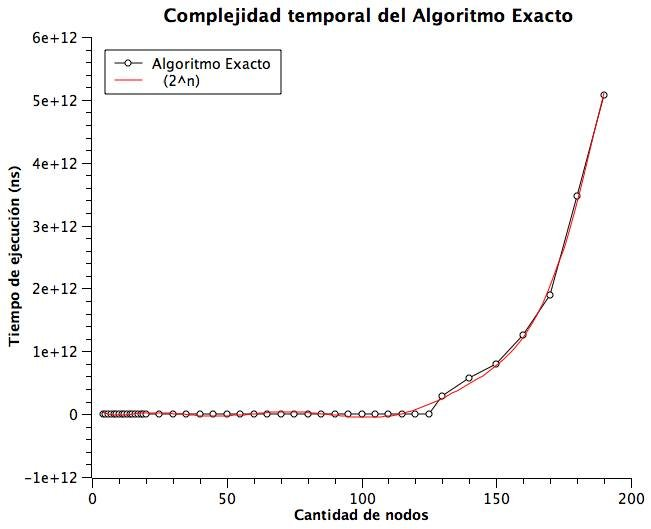
\includegraphics[width=350pt]{../imgs/exactoComplejidad.jpg}
\end{center}
\end{figure}

Como puede observarse en el gráfico anterior, la complejidad de nuestro algoritmo exacto se encuentra acotada por una función exponencial.

\newpage

\section{Heurística Golosa}
\subsection{Explicación del algoritmo realizado}
Para resolver el algoritmo presentado anteriormente con una técnica golosa, decidimos utilizar el procedimiento que se presenta a continuación:\newline
\newline
\begin{algorithm}[H]
    \SetAlgoLined
    \caption{HeurísticaGolosa}
    \KwIn{\textbf{Grafo} $g$}
    \KwOut{\textbf{Conj(nodos)} $clique$}
	Entero $nodoDeMayorGrado$ = nodoDeMasGrado($g$)\\
	Grafo $cliqueHastaAhora$ = $\emptyset$\\
	agregar($v$, $cliqueHastaAhora$)\\
	\ForAll{$u \in$ adyacentes(nodoDeMayorGrado, nodos($g$))}{
		\If{forma una clique($g$, agregar($u$, $cliqueHastaAhora$)) $\land$ frontera($g$, agregar($u$, $cliqueHastaAhora$) $>$ frontera($cliqueHastaAhora$)}{
		agregar($u$, $cliqueHastaAhora$)}}
\textbf{devolver} $cliqueHastaAhora$
\end{algorithm}

donde $nodoDeMasGrado$ consiste en una función que toma el nodo del grafo cuyo grado es el mayor, $frontera$ es una función que calcula la frontera de un conjunto de nodos dentro de un grafo y $adyacentes$ consiste en una lista de nodos adyacentes a un determinado nodo.\newline


\subsection{Complejidad Temporal}
Veamos cuál es la complejidad temporal del algoritmo realizado:
\begin{itemize}
\item En primer lugar, el algoritmo utiliza la función $esClique$ para verificar si un conjunto de nodos de un grafo forman una clique. Dicha función consiste en dos ciclos, uno dentro de otro, que iteran cantidad de la clique veces, lo que resulta $\mathcal{O}(n^2)$ como peor caso. Dentro de los ciclos mencionados, se realizan dos comparaciones, donde una de ellas utiliza la función $sonVecinos$ ($\mathcal{O}(1)$). Luego, la complejidad temporal de la función $esClique$ resulta $\mathcal{O}(n^2)*\mathcal{O}(1)$ = $\mathcal{O}(n^2)$.

\item Por otro lado, la función $greedySearch$ crea un vector inicializado en 1 de tamaño $nodoDeMayorGrado$ ($\mathcal{O}(n)$) y un entero al que se le asigna el valor de la frontera de $cliqueHastaAhora$. Dicho valor se calcula con $frontera$ en $\mathcal{O}(n)$. Luego, se ejecuta un ciclo con la cantidad de nodos ($\mathcal{O}(n)$) en el que se realiza un $push\_back$ ($\mathcal{O}(1)$ amortizado\footnote{http://www.cplusplus.com/reference/vector/vector/push\_back/}) y se verifica que el vector $cliqueHastaAhora$ sea una clique con la función $esClique$ ($\mathcal{O}(n^2)$). Si dicha verificación resulta afirmativa, se compara la frontera de $cliqueHastaAhora$ con un entero ($\mathcal{O}(n)$) y luego se le asigna la nueva frontera a $fronteraHastaAhora$ (con la función $frontera$ en $\mathcal{O}(n)$). Caso contrario, se retira el último elemento agregado a la clique con $pop\_back()$ ($\mathcal{O}(1)$\footnote{http://www.cplusplus.com/reference/vector/vector/pop\_back/}).\newline
\newline
Luego, la complejidad temporal de la función $greedySearch$ resulta $2^*\mathcal{O}(n)+\mathcal{O}(n)^*\mathcal{O}(n)^*\mathcal{O}(n^2)$ = $\mathcal{O}(n^4)$.

\end{itemize}
\subsection{Instancias problemáticas}
Este algoritmo siempre parte del nodo de mayor grado y siempre agrega nodos, es decir, nunca quita, por lo que si la solucion optima no contiene dicho nodo entonces nunca se va a encontrar el mejor caso. \newline
 Esto genera que uno pueda crear un caso tan malo como quiera, solo se necesita poner un nodo con grado $d$ y otras cliques que posean grado $d-1$ de forma tal que la frontera de dichas cliques sea mayor a $d$.
 
\subsection{Experimentación}
Para la experimentación de la Heurística Golosa, nos limitamos a realizar un gráfico comparativo para grafos aleatorios entre la cantidad de nodos agregados respecto del tiempo de ejecución. Para ello, utilizamos un generador de grafos y aumentamos de forma paulatina la cantidad de nodos, respetando una densidad del 50\% para las aristas.\newline
Las mediciones de tiempo en nanosegundos se realizaron con la función $high\ resolution\ clock$\footnote{http://en.cppreference.com/w/cpp/chrono/high\_resolution\_clock} de la librería $Chrono$ de $C++$. 

Las funciones de complejidad con las que se compararon nuestros gráficos de tiempo fueron ajustadas por algoritmos matemáticos (proporcionados por \textbf{sci davis}). Dichos algoritmos se encargaron de multiplicarle y sumarle constantes a las funciones con el fin de que éstas se ajustaran a nuestros resultados sin modificar el comportamiento de las funciones utilizadas para comparar.

\begin{figure}[H] %[h] Aqui [b] para button [t] para top
\begin{center}
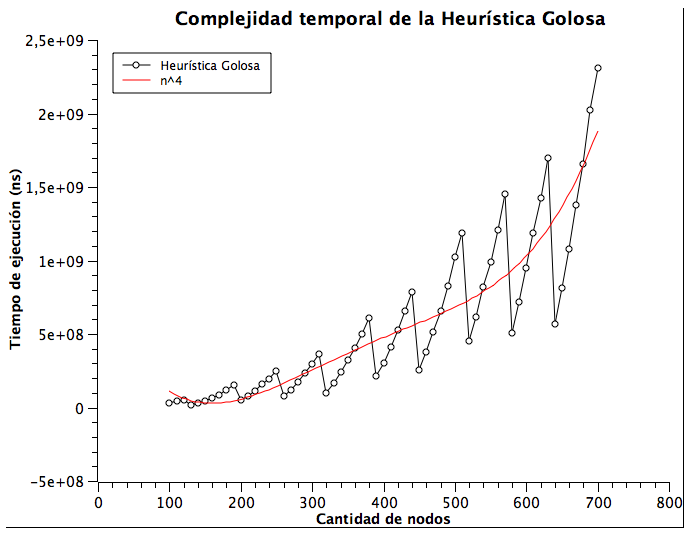
\includegraphics[width=350pt]{../imgs/complejidad_goloso.png}
\caption{Complejidad Temporal de la Heurística Golosa.}
\end{center}
\end{figure}


\newpage

\section{Heurística de Búsqueda Local}
\subsection{Explicación del algoritmo realizado}
Los algoritmos de búsqueda local parten de una solución inicial $S_{0}$ y en cada paso intentan mejorarla. Para esto, una opción consiste en calcular todas las posibles variaciones de $S_{0}$ que forman una solución al problema. Al conjunto de todas estas se lo llama vecindad. 
Estos algoritmos se ejecutan siempre y cuando exista una solución, perteneciente a la vecindad, que sea mejor a la ya obtenida.\newline
\newline
Para nuestro ejercicio, utilizamos como $S_{0}$ al nodo de mayor grado. Dicha elección se debió a que un nodo forma una clique, con lo cual es una posible solución a nuestro problema. Además, sabemos que éste existe para cualquier grafo ya que la menor cantidad de nodos que se puede ingresar en nuestro programa es uno. 
\newline Por otro lado, decidimos definir como vecindad a todas las posibles cliques que difirieran en a lo sumo un nodo con nuestro $S_{0}$. Esta decisión la tomamos para que nuestra clique no quedara fija alrededor del nodo inicial. Para evitar tener que almacenar todas las posibles cliques para, posteriormente, elegir la mejor, decidimos separar la vecindad en tres subconjuntos. Estos se formaron con las cliques que cumplen lo siguiente:
\begin{itemize}
\item \textbf{Tiene todos los nodos de $S_{0}$ salvo 1:} \newline En lugar de calcular todas las posibles cliques de este subconjunto, decidimos quedarnos únicamente con la clique que se obtiene de quitarle el nodo de menor grado a $S_{0}$. Esto se debe a que la frontera de una clique se puede calcular con la siguiente formula:\newline
Sea $S_{0}$ = ($V$,$E$) y n = $|$$V$$|$
\begin{equation}
  \delta(S_{0}) = \sum_{v \in V}^{} d(v) - n*(n-1)
\end{equation}
Ahora, si quitamos un nodo $v'$ de $S_{0}$, obtenemos lo siguiente:
\begin{equation}
  \delta(S'_{0}) = \sum_{v \in V/v'}^{} d(v) - (n-1)*(n-2)
\end{equation}
Dado que se desea encontrar el mayor \delta$(S'_{0})$, se debe guardar el que tiene la sumatoria de mayor valor ya que (n-1)*(n-2) es igual para todas las cliques. Con lo cual, el nodo que debemos eliminar para poder maximizar la sumatoria, es el de menor grado.

El pseudo código de este subconjunto de la vecindad es:\newline
\begin{algorithm}[H]
    \SetAlgoLined
    \caption{quitarNodo}
    \KwIn{\textbf{Grafo} $grafo$, \textbf{Conj(Entero)} $clique$}
    \KwOut{\textbf{par(Entero,Conj(Entero))} $res$}
	
    \textbf{Entero} $minimo$ = $|$vecindad(0)$|$ \\	
    \textbf{Entero} $minimoNodo = 0$ \\
    \ForAll{$v \in$ $|clique|$}{
        $tamañoVecindad$ = $|$vecindad($v$)$|$ \\
		\If{$tamañoVecindad < minimo$}{
            $minimo$ = $tamañoVecindad$ \\
			$minimoNodo$ = $v$
	 		}}
    
    \textbf{Conj(Entero)} $cliqueQuitando$\\

    \ForAll{$v \in$ $|clique|$}{
		\If{$v \neq minimoNodo$}{
            agregar($cliqueQuitando$, $v$)
	 		}}
    
    \textbf{Entero} $fronteraRes$ = frontera($grafo$, $cliqueQuitando$)\\
    $res$ = hacerPar($fronteraRes$, $cliqueQuitando$)\\
    \textbf{devolver} $res$ \\
\end{algorithm}

Donde $frontera$ calcula la frontera del subgrafo pasado por parámetro, $agregar$ inserta un elemento en un arreglo, $vecindad$ nos devuelve todos los nodos adyacentes al nodo pasado por parámetro y $hacerPar$ genera un par con lo dos elementos pasados por parámetro. \newline


\item \textbf{Tiene todos los nodos de $S_{0}$ más uno que no pertenecía a el:} \newline
Para poder obtener la clique de frontera máxima de este subconjunto, buscamos todos los nodos del grafo que pueden formar una clique con $S_{0}$. Para esto, contamos cuantos nodos de la clique se conectan a cada nodo del grafo. Si un nodo es alcanzado por todos los que pertenecen a $S_{0}$, entonces al agregarlo, $S_{0}$ seguiría formando una clique. Una vez que tenemos a todos los posibles candidatos, calculamos la frontera de cada uno y nos quedamos con la mayor. \newline

\begin{algorithm}[H]
    \SetAlgoLined
    \caption{agregarNodo}
    \KwIn{\textbf{Grafo} $grafo$, \textbf{Conj(Entero)} $clique$}
    \KwOut{\textbf{par(Entero,Conj(Entero))} $res$}
	
    \textbf{Conj(Entero)} $adyacentesPorCadaNodo[|$Nodos($grafo$)$|]$  \\
	
    $adyacentesPorCadaNodo$ = marcarNodos
	
    \textbf{Conj(Nodo)} $posibleClique$ = dameCandidatosAClique($adyacentesPorCadaNodo$)\\
   
    \textbf{Entero} $maxFrontera = 0$ \\
    \textbf{Entero} $nodo = 0$ \\

    \ForAll{$v \in$ Nodos($posibleClique$)}{
	agregar($clique$, $v$) \\
		\If{frontera($clique$) $> maxFrontera$}{
		    $maxFrontera = $ frontera($clique$)\\
		    $nodo = v$
	}
	quitar($clique$, $v$) \\}


    \eIf{ $|posibleClique| =$ 0}
	{$res$ = hacerPar(0, $clique$)}
    {	agregar($clique$, $v$) \\
	$res$ = hacerPar($maxFrontera$, $clique$) }

    \textbf{devolver} $res$ \\
\end{algorithm}

Donde $marcarNodos$ calcula para cada nodo, cuantos nodos de la clique son adyacentes a el, $dameCandidatosAClique$ nos devuelve los nodos de marcarNodos que fueron marcados por todos los nodos de la clique, $frontera$ calcula la frontera del subgrafo pasado por parámetro, $Nodos$ devuelve todos los nodos del subgrafo, $agregar$ inserta un elemento en un arreglo, $quitar$ quita un elemento en un arreglo, $vecindad$ nos devuelve todos los nodos adyacentes al nodo pasado por parámetro y $hacerPar$ genera un par con lo dos elementos pasados por parámetro. \newline

\item \textbf{Tiene todos los nodos de $S_{0}$ salvo 1 que se lo reemplaza por otro que no estaba en el:} \newline
En este subconjunto lo primero que hicimos fue quitar un nodo de $S_{0}$ y posteriormente, con la clique que nos quedo, agregarle otro. Para esto, utilizamos las funciónes quitarNodo y agregarNodo. Al hacer esto, logramos que nuestra clique no quede centrada en el nodo de mayor grado ya que este eventualmente podría dejar de formar parte de la solución y ser permutado por otro.\newline
En el caso de que $S_{0}$ tenga un solo elemento, al aplicar quitarNodo, la funcion nos devuelve un grafo vacio. Si esto sucede, decidimos agregar el nodo de mayor grado de todos los adyacente al unico que estaba en $S_{0}$. Esto lo hicimos ya que agregarNodo no puede recibir una clique vacia.\newline
Si por el contrario quitarNodo nos devuelve un grafo, aplicamos la funcion agregarNodo sobre este. \newline
Como quitarNodo y agregarNodo son dos funciones distintas, es posible que al aplicar ambas obtengamos el mismo $S_{0}$. En el caso de que esto suceda, no habría problema ya que significaría que de todas las cliques de este subconjunto, ninguna tiene mayor frontera que $S_{0}$. Por otro lado, el resultado que obtenemos es una clique ya que quitarNodo devuelve una clique o un conjunto vacio. Si devuelve una clique, usamos agregarNodo que tambien nos devuelve una clique. Caso contrario, generamos una clique con un unico nodo.
\begin{algorithm}[H]
    \SetAlgoLined
    \caption{permutarNodo}
    \KwIn{\textbf{Grafo} $grafo$, \textbf{Conj(Entero)} $clique$}
    \KwOut{\textbf{par(Entero,Conj(Entero))} $res$}
	
   \textbf{Conj(Entero)} $cliqueParcial$ = segundo(quitarNodo($grafo$, $clique$)) \\

    \eIf{$cliqueParcial = \emptyset$}{
	    \textbf{Entero} $nodo$ = vecinoDeMayorGrado($grafo$,$clique$) \\
            agregar($cliqueParcial$, $nodo$)\\
	    $res$ = hacerPar (frontera($cliqueParcial$), $cliqueParcial$)	
	 		}{$cliqueParcial$ = agregarNodo($grafo$, $cliqueParcial$)\\
	 		 $res$ = hacerPar (frontera($cliqueParcial$), $cliqueParcial$)
	 		}

    \textbf{devolver} $res$ \\
\end{algorithm}
Donde $segundo$ nos devuelve el segundo elemento de una tupla,  $agregar$ inserta un elemento en un arreglo, $vecinoDeMayorGrado$ nos da el nodo de mayor grado entre todos los vecinos del vértice pasado por parámetro, $frontera$ calcula la frontera del subgrafo pasado por parámetro, $vecindad$ nos devuelve todos los nodos adyacentes al nodo pasado por parámetro y $hacerPar$ genera un par con lo dos elementos pasados por parámetro. \newline
\end{itemize}

Una vez que generamos a los tres candidatos de la vecindad, tomamos al que tiene mayor frontera y lo comparamos con $S_{0}$. Si la frontera de $S_{0}$ es menor, entonces la clique de frontera máxima de nuestra vecindad es nuestra nueva solución inicial. Caso contrario, el programa finaliza ya que ningún elemento de la vecindad puede mejorarla.

\subsection{Complejidad Temporal}
Para analizar la complejidad de nuestro algoritmo, vamos a separarlo en 5 funciones:
\begin{itemize}
\item \textbf{Generar grafo:} \newline
Para poder obtener la mayoría de las operaciones que utilizan nuestras funciones en $\mathcal{O}(1)$, generamos el grafo con los parámetros de entrada, utilizando lista y matriz de adyacencia. De esta forma, evitamos aumentar la complejidad de nuestro algoritmo. Por consiguiente, la complejidad es $\mathcal{O}(n^{2})$ ya que este es el costo de crear la matriz de adyacencia.

\item \textbf{quitarNodo:} \newline
Como podemos observar en el pseudocódigo de la función $quitarNodo$, lo primero que hace nuestro algoritmo es calcular mediante la función $vecindad$ ($\mathcal{O}(1)$) de la clase grafo, el tamaño de la vecindad del nodo 0. Posteriormente, hay un ciclo el cual consiste en recorrer todos los nodos de la clique($\mathcal{O}(n)$) y almacenar el de menor grado en cada paso ($\mathcal{O}(1)$).
\newline
Luego, hay un ciclo el cual nuevamente recorre todos los nodos de la clique ($\mathcal{O}(n)$) y en cada paso utiliza la función $agregar$ la cual fue implementada con $push\_back$\footnote{http://www.cplusplus.com/reference/vector/vector/push\_back/} con una complejidad de $\mathcal{O}(1)$.
\newline
Por ultimo, se calcula el valor de la frontera mediante la función $frontera$ de la clase grafo, la cual tiene una complejidad de $\mathcal{O}(n)$ y se genera un par con la solución del problema. Este par es generado mediante la función $make\_pair$\footnote{http://www.cplusplus.com/reference/utility/make\_pair/} cuya complejidad es $\mathcal{O}(1)$.
\newline
Como se puede observar, la complejidad final de $quitarNodo$ es $\mathcal{O}(n)$

\item \textbf{agregarNodo:} \newline 
Como podemos observar en el pseudocódigo de la función $agregarNodo$, lo primero que hace nuestro algoritmo es crear un arreglo de $n$ posiciones ($\mathcal{O}(n)$). Posteriormente, hace $marcarNodos$ el cual para cada nodo de la clique($\mathcal{O}(n)$), se fija cuales son sus vecinos mediante la función $vecindad$ ($\mathcal{O}(1)$) de la clase grafo. Luego, para cada uno de estos, ($\mathcal{O}(n)$) le suma uno a la cantidad de nodos adyacentes perteneciente a la clique que poseen. Por lo tanto, la complejidad de $marcarNodos$ es $\mathcal{O}(n^{2})$. \newline
Una vez que calcula cuantos nodos de la clique son adyacentes a cada nodo del grafo, hace $dameCandidatosAClique$. Esta función toma todos los nodos del grafo y se fija para cada uno de ellos ($\mathcal{O}(n)$) si el valor que calculo $marcarNodos$ es igual al tamaño de la clique, el cual, es calculado mediante la función size($\mathcal{O}(1)$). Por lo tanto su complejidad es ($\mathcal{O}(n)$). \newline
Posteriormente, a cada nodo de $dameCandidatosAClique$ ($\mathcal{O}(n)$), lo agrega a $S_{0}$, mediante la función $push\_back$,\footnote{http://www.cplusplus.com/reference/vector/vector/push\_back/}($\mathcal{O}(1)$). Luego, compara la frontera ($\mathcal{O}(n)$) de esta nueva clique con la frontera mas grande hasta el momento. En caso de que esta sea mayor, almacena que nodo fue el que agrego y cual es el valor de su frontera. Por ultimo, quita este nodo mediante la función $pop\_back$\footnote{http://www.cplusplus.com/reference/vector/vector/pop\_back/} cuya complejidad es $\mathcal{O}(1)$). El costo de realizar esto es $\mathcal{O}(n^{2})$. \newline
Una vez que tiene la solución, genera un par con esta mediante la función $make\_pair$\footnote{http://www.cplusplus.com/reference/utility/make\_pair/} cuya complejidad es $\mathcal{O}(1)$.
\newline
Como se puede observar, la complejidad final de $agregarNodo$ es $\mathcal{O}(n^{2})$

\item \textbf{permutarNodo:} \newline 
Como podemos observar en el pseudocódigo Nº 8, nuestro algoritmo hace dos cosas. Primero le quita un nodo a la clique mediante la función $quitarNodo$ cuya complejidad es $\mathcal{O}(n)$. Posteriormente, se fija si el resultado de $quitarNodo$ es vacío o no. \newline
En el caso de que sea vacío, calcula mediante $vecinoDeMayorGrado$ cual de todos los nodos adyacentes al pasado por parámetro tiene mayor grado. Para esto, recorre todos los nodos adyacentes y compara en $\mathcal{O}(1)$ sus grados, por lo tanto su complejidad es $\mathcal{O}(n)$. Una vez que tiene la solución, la coloca en un arreglo mediante $push\_back$ y genera un par con esta mediante la función $make\_pair$ cuya complejidad es $\mathcal{O}(1)$.
\newline
Si por el contrario, la clique no estaba vacía, obtiene la solución mediante la función $agregarNodo$ cuya complejidad es $\mathcal{O}(n^{2})$
\newline
Como se puede observar, la complejidad final de $permutarNodo$ es $\mathcal{O}(n^{2})$

\item \textbf{busquedaLocal:} \newline 

\begin{algorithm}[H]
    \SetAlgoLined
    \caption{busquedaLocal}
    \KwIn{\textbf{Grafo} $grafo$, \textbf{Entero} $m$}
    \KwOut{\textbf{Conj(Entero)} $res$}
	
    agregar($res$, nodoDeMayorGrado($grafo$))\\
    	
    \For{i = 0  \textbf{to} i $<$ m}{
        \textbf{par(Entero, Conj(Entero))} $solucionParcial = $ agregarNodo($grafo, res$)\\
	\If{primero($solucionParcial$)$ < $primero(quitarNodo($grafo$, $res$))}{
            $solucionParcial = $ quitarNodo($grafo$, $res$)\\
	 		}
    	\If{primero($aux$)$ < $primero(permutarNodo($grafo$, $res$))}{
            $solucionParcial = $ permutarNodo($grafo$, $res$)\\
	 		}
	\eIf{primero($solucionParcial$)$ > $frontera($res$)}{
            $res = $ primero($solucionParcial$)\\
	 		}{$salir del ciclo$}
	}
    \textbf{devolver} $res$ \\
\end{algorithm}

Como se observa en el pseudocódigo Nº 9, nuestro algoritmo coloca en $res$ el nodo de mayor grado del grafo. Esta función tiene complejidad $\mathcal{O}(n)$.
Posteriormente, utiliza las funciones agregarNodo ($\mathcal{O}(n^{2})$), quitarNodo ($\mathcal{O}(n)$) y permutarNodo ($\mathcal{O}(n^{2})$). Estas tres funciones se encuentran dentro de un ciclo el cual itera como máximo $m$ veces. La razon por la cual la cantidad de iteraciones esta acotada por la cantidad de aristas es la siguiente:\newline
Como explicamos al comienzo, el algoritmo de busqueda local consiste en partir de una solucion inicial y en cada paso mejorarla. Esto significa que nuestro ciclo deberia iterar hasta encontrar la mejor solucion posible y una vez ayada dejar de ciclar. En nuestro caso, las soluciones parciales son cliques de frontera maxima. Esto quiere decir que en cada paso se intenta mejorar la cantidad de aristas que posee la clique perteneciente a la solucion anterior. Supongamos ahora que la solucion inicial con la cual ingresamos al ciclo posee frontera igual a 1. Por otro lado, supongamos tambien que en cada iteracion del ciclo, se encuentra una solucion que mejora en uno a la que se tenia. Si  esto ocurre, en cada iteracion se iria agregando una arista, con lo cual no seria necesario que nuestro ciclo itere más de $m$ veces, ya que es la cantidad maxima de aristas que puede agregar. Es por esto que nuestro algoritmo encuentra la mejor solucion posible en a lo sumo $m$ pasos. Por ultimo, la complejidad del ciclo es $\mathcal{O}(n^{2})$ * $\mathcal{O}(n^{2})$                                                                        
                                                                                
\newline
Como se puede observar, la complejidad final de $busquedaLocal$ es $\mathcal{O}(n^{4})$.
\end{itemize}
\subsection{Instancias problemáticas}
Si observamos nuestro algoritmo, podemos notar que este siempre arranca por el nodo de mayor grado. Posteriormente, se va moviendo, en cada iteración, a una clique la cual dista a lo sumo en una unidad con la clique actual. Teniendo en cuenta esto, nuestro algoritmo va a encontrar la solución exacta siempre y cuando haya cliques, las cuales generen fronteras cada vez mas grande, entre el nodo de mayor grado y la clique de frontera máxima.
\newline
Veamos que sucede en el caso en el que la solución no es la óptima. Como ya dijimos antes, partimos del nodo de grado máximo, por lo tanto d($S_{0}$) $\leq$ frontera($S$). Por otro lado, se que los grados de los nodos que conforman $S$ no pueden ser mayores a d($S_{0}$). Esto se debe a que si lo fueran, estos serian el $S_{0}$ de nuestro algoritmo. Como quiero ver que tan mala es la solución que obtuve, voy a buscar la solución con máxima frontera. Para esto, calculemos cuanto vale la frontera de una clique genérica. \newline
En primer lugar, notemos que para maximizar la frontera, debemos tener todos los nodos de la clique con la mayor cantidad de aristas posibles. Como vimos anteriormente, el grado de los nodos no puede superar a d($S_{0}$). Luego, para una clique de $c$ nodos de grado d($S_{0}$), obtenemos que su frontera es:
\begin{equation}
  frontera(S) = d(S_{0}) * c - (c - 1) * c
\end{equation} 
Esta es la frontera mas grande que se puede encontrar para cada valor de $c$.
\newline 
Ahora, veamos cuanto es el máximo error que se puede cometer al no encontrar la solución óptima. Para esto, debemos restarle a la formula anterior d($S_{0}$). Esto se debe a que es la menor frontera que encuentra nuestro algoritmo.
\begin{equation}
  máximo\ error = d(S_{0}) * c - (c - 1) * c - d(S_{0}) 
\end{equation} 
Saco factor común d($S_{0}$)
\begin{equation}
  máximo\ error = d(S_{0}) * (c - 1) - (c - 1) * c 
\end{equation} 
Saco factor común (c - 1)
\begin{equation}
  máximo\ error = (c - 1) * (d(S_{0}) - c) 
\end{equation} 
Calculemos cual es el valor de c que maximiza esta función. Derivemos con respecto a $c$
\begin{equation}
  máximo\ error' = (d(S_{0}) - c) - (c - 1)
\end{equation} 
igualemos a 0 y despejemos
\begin{equation}
  c = \frac{1 + d(S_{0})}{2}
\end{equation} 
Si derivo una vez mas y evalúo en c = $\frac{1 + d(S_{0})}{2}$, obtengo que:
\begin{equation}
  máximo\ error'' = -2 < 0
\end{equation}
Por lo tanto es máximo.\newline \newline
Veamos cual es el máximo error que se puede obtener.

\begin{equation}
  máximo\ error = d(S_{0}) * \frac{1 + d(S_{0})}{2} - (\frac{1 + d(S_{0})}{2} - 1) * \frac{1 + d(S_{0})}{2} - d(S_{0}) 
\end{equation} 
\begin{equation}
  máximo\ error = \frac{1 - 2 * d(S_{0}) + d(S_{0})^{2}}{4} 
\end{equation}

veamos 2 casos en donde nuestro algoritmo no encuentra la solución óptima:
\begin {itemize}
\item
\textbf{Formato de entrada:}

$$14\ \  14$$
$$1\ \  2$$
$$1\ \  3$$
$$1\ \  4$$
$$1\ \  5$$
$$1\ \  6$$
$$6\ \  7$$
$$7 \ \ 8$$
$$8\ \  9$$
$$9\ \  7$$
$$8\ \  10$$
$$8\ \  11$$
$$9\ \  12$$
$$9\ \  13$$
$$7\ \  14$$


\textbf{Formato de salida:}
$$5\ \   1\ \   1$$
\begin{figure}[H] %[h] Aqui [b] para button [t] para top
\begin{center}
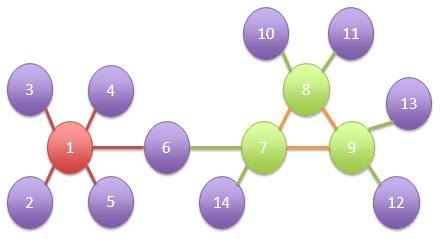
\includegraphics[width=250pt]{../imgs/ej1local.jpg}
\caption{Ejemplo}
\end{center}
\end{figure}
Como se puede notar en el grafico, la frontera máxima según nuestro algoritmo es 5 (aristas rojas) cuando la exacta es en realidad 6 (aristas verdes) y esta conformada por los nodos 7 8 9 . esto se debe a que el nodo de mayor grado es el 1 y dista en dos nodo de la clique máxima. 
\newline
comprobemos que esto satisface nuestra cota:
\begin{equation}
  máximo\ error = \frac{1 - 2 * 5) + 5^{2}}{4} = 4
\end{equation}
\begin{equation}
  algoritmo\ exacto - heurística = 6 - 5 = 1
\end{equation}

\item
\textbf{Formato de entrada:}

$$17\ \  17$$
$$1\ \  2$$
$$1\ \  3$$
$$1\ \  4$$
$$1\ \  5$$
$$1\ \  6$$
$$6\ \  7$$
$$7 \ \ 8$$
$$8\ \  9$$
$$9\ \  7$$
$$8\ \  10$$
$$8\ \  11$$
$$9\ \  12$$
$$9\ \  13$$
$$7\ \  14$$
$$7\ \  15$$
$$8\ \  16$$
$$9\ \  17$$

\textbf{Formato de salida:}
$$5\ \   1\ \   1$$
\begin{figure}[H] %[h] Aqui [b] para button [t] para top
\begin{center}
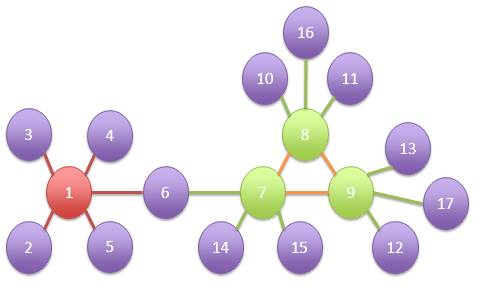
\includegraphics[width=250pt]{../imgs/ej2local.jpg}
\caption{Ejemplo}
\end{center}
\end{figure}
Como se puede notar en el gráfico, la frontera máxima según nuestro algoritmo es 5 (aristas rojas) cuando la exacta es en realidad 9 (aristas verdes) y esta conformada por los nodos 7 8 9 . esto se debe a que el nodo de mayor grado es el 1 y dista en dos nodo de la clique máxima.
\newline
comprobemos que esto satisface nuestra cota:
\begin{equation}
  máximo\ error = \frac{1 - 2 * 5 + 5^{2}}{4} = 4
\end{equation}

\begin{equation}
  algoritmo\ exacto - heurística = 9 - 5 = 4
\end{equation}
\end{itemize}

\subsection{Experimentación}

\begin{figure}[H] %[h] Aqui [b] para button [t] para top
\begin{center}
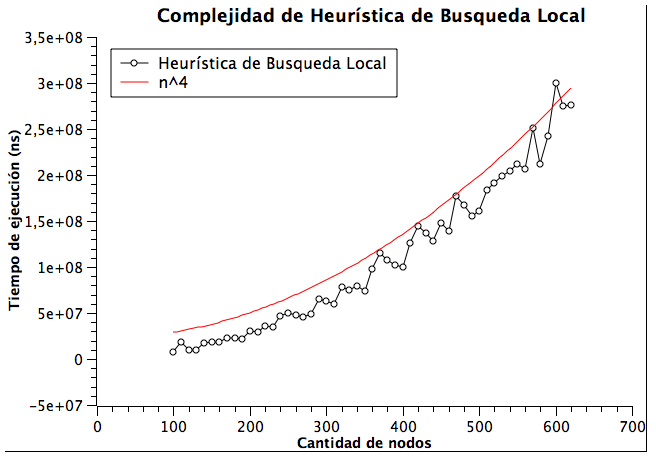
\includegraphics[width=350pt]{../imgs/complejidad_local.png}
\caption{Complejidad Temporal de la Heurística de Búsqueda Local.}
\end{center}
\end{figure}

\newpage
\section{Metaheurística de Búsqueda Tabú}
En esta sección, se busca resolver el problema de CMF a partir de una Heurística de Búsqueda Tabú (Tabu search\footnote{Glover, F. "Tabu Search — Part I", ORSA Journal on Computing 1989}). Dicha heurística consiste en una estrategia para resolver problemas combinatorios, aplicable tanto en grafos como en otras estructuras utilizadas para resolver problemas de lógica. Este método utiliza el mismo procedimiento que Búsqueda Local\footnote{Ver sección anterior.} para acercarse progresivamente a una mejor solución dentro de un entorno. Dado que en ciertos casos la solución no puede ser mejorada, la técnica de Búsqueda Tabú permite empeorarla parcialmente para proseguir la búsqueda de una mejor. A su vez, esta heurística concede una estructura llamada $lista\ tabú$ con distintas utilidades. Principalmente, sirve para guardar movimientos de modo a no repetirlos y/o guardar características o soluciones, entre otras. A continuación, se encuentra explicitado el pseudocódigo\footnote{http://www.dc.uba.ar/materias/aed3/2013/2c/laboratorio/heuristicas.pdf} de la heurística de Búsqueda Tabú:

\begin{algorithm}[H]
\SetAlgoLined
s$_{0}$ $\leftarrow$ solucion inicial \\
s$^{*}$ $\leftarrow$ s$_{0}$ \\
T $\leftarrow$ lista tabú inicial \\
\While{ no se alcance el criterio de terminacion}{
N $\leftarrow$ vecinos de s no tabú o mejores que s$^{*}$ \\
s $\leftarrow$ mejor solucion en N. \\
\If{ s es mejor que s$^{*}$}
 {s$^{*}$ $\leftarrow$ s} 
Actualizar la lista tabú T }
\end{algorithm}

\subsection{Explicación del algoritmo realizado}

 El algoritmo realizado parte de un valor entero positivo ingresado como parámetro, $desviacion\_permitida$, y de una solución provista por la Heurística de Búsqueda Local. A partir de esta última, el algoritmo busca, paulatinamente, una mejor solución siguiendo las siguientes opciones:
\begin{itemize}
 \item Agregando un nodo: Dada la solución actual (una clique), procede a $agregar$ un nodo que la mejore, es decir, que aumente su frontera.
 \item Quitando un nodo: Dada la solución actual (una clique), procede a $quitar$ un nodo que la mejore, es decir, que aumente su frontera.
\end{itemize}
A diferencia de la Búsqueda Local, se buscan nuevas soluciones que no necesariamente mejoren la solución obtenida hasta el momento pero que sí lo hagan a largo plazo. Sin embargo, dentro de las formas de empeorar la solución, se toma aquella que empeora lo menos posible. A su vez, a medida que se agrega o quita un nodo, se lo inserta en la lista tabú. Esto se realiza sin olvidar que siempre que pueda subir lo va a hacer, entonces, si descendiendo se encuentra con que puede volver a ascender, lo va a hacer hasta volver a estar en un máximo local.\newline

\begin{figure}[H] %[h] Aqui [b] para button [t] para top
\begin{center}
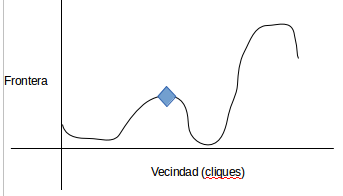
\includegraphics[width=250pt]{../imgs/1_tabu.png}
\caption{solución con Busqueda Local}
\subcaption{Aqui se muestra en el dominio la vecindad y en la imagen el valor de la frontera. El rombo rojo representa la solucion de la Busqueda Local.}
\end{center}
\end{figure}


\begin{figure}[H] %[h] Aqui [b] para button [t] para top
\begin{center}
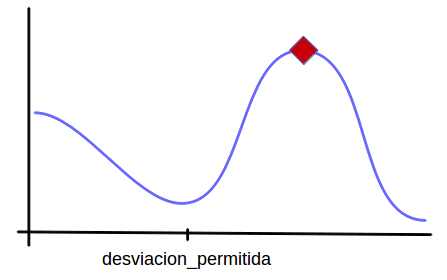
\includegraphics[width=250pt]{../imgs/2_tabu.png}
\caption{solución con Busqueda tabú}
\subcaption{Este es el mismo grafico anterior pero se puede notar como despues de aplicar $desviacion_permitida$ "descensos" la solucion comienza a mejorar hasta para en otro maximo local (mejor que el dado por Busqueda Local).}
\end{center}
\end{figure}

Al finalizar, el algoritmo retorna la mejor solución hallada. \newline

\textbf{Descripción de la lista tabú} \newline

 A medida que se van agregando o quitando nodos que no mejoran la solución, se los va marcando como tabú. De esta forma, se le asigna una prioridad a cada uno de ellos que depende del momento en que fue agregado. A su vez, sea cual sea la prioridad del último nodo insertado, éste no puede utilizarse en la iteración siguiente para evitar ciclar soluciones. Para lograr esto, hicimos que en el peor de los casos sólo se puedan usar los nodos tabús que tienen prioridad menor a la mitad de la prioridad máxima. Las ventajas de esto es que evitamos ciclar con los mismos nodos (por ejemplo, agregando y quitando un nodo) y a su vez permite trabajar con nodos de manera mas dispersa y no siempre con los mismos. Las desventajas es que cuando uno realiza una operación $p$ con un nodo $u$, y había otra operación $p'$ que aplicada al nodo $u$ producía menos frontera, se va a elegir realizar la operación $p$, pero por ahí para llegar a la optima había que realizar la operación $p'$ y esto no se va a realizar a corto plazo ya que el nodo es puesto como tabú.\newline

\textbf{Criterio de terminación} \newline

 El algoritmo presentado tiene dos criterios de terminación. Por un lado, la cantidad de iteraciones en que la solución puede mejorar y, por el otro, la variable $desviacion\_permitida$ ingresada como parámetro. El primero se encuentra acotado por el máximo absoluto que existe pues el problema siempre tiene solución. Luego, pueden existir muchos máximos locales pero ninguno será una clique con mayor frontera que la del máximo absoluto (esto resulta trivial). Por otro lado, la variable $desviacion\_permitida$ va disminuyendo cada vez que se modifica la solución actual sin mejorarla, es decir, que permitimos avanzar de manera ``no creciente'' una cantidad $desviacion\_permitida$ de veces. \newline




\begin{algorithm}[H]
    \SetAlgoLined
    \caption{TabuSearch}
    \KwIn{\textbf{Conj(nodos)} $solución\_inicial$, \textbf{Grafo} $g$, \textbf{Entero} $desviacion\_permitida$}
    \KwOut{\textbf{Conj(nodos)} $solución\_final$}

	\textbf{Conj(nodos)} sol$_{0}$,sol$_{1}$ \\ 
	\textbf{Conj(nodos)} $solución\_actual$ $\leftarrow$ LocalSearch($solución\_inicial$, $g$)	\\	
	\textbf{Conj(nodos)} $solución\_final$ $\leftarrow$ $solución\_actual$	\\	
	\textbf{Lista Tabu} $\leftarrow$ $\{\}$\\
	\textbf{Boolean} $Mejore\ la\ frontera$ $\leftarrow$ true

	\While{ $Mejore\ la\ frontera$ $\vee$ 0 $<$ $desviacion\_permitida$}{

	 	sol$_{0}$ $\leftarrow$ Dame Mejor solución agregando nodo No Tabu ($solución\_inicial$,$solución\_final$) \\
		sol$_{1}$ $\leftarrow$ Dame Mejor solución quitando nodo No Tabu ($solución\_inicial$,$solución\_final$) \\
		\If{ frontera(sol$_{0}$) $<$ frontera(sol$_{1}$)}
			{sol$_{0}$ $\leftarrow$ sol$_{1}$}
		\eIf{ frontera($solución\_actual$) $<$ frontera(sol$_{1}$)}
			{$solución\_actual$ $\leftarrow$ sol$_{0}$ \\
			$Mejore\ la\ frontera$ $\leftarrow$ true
			}
			{$Mejore\ la\ frontera$ $\leftarrow$ false \\
			 Poner Tabu Nodo utilizado en sol$_{0}$ \\
			 $desviacion\_permitida$ = $desviacion\_permitida$ - 1}
		$solución\_actual$ $\leftarrow$ sol$_{0}$ \\
		\If{ frontera($solución\_final$) $<$ frontera($solución\_actual$) } 
		{$solución\_final$ $\leftarrow$ $solución\_actual$}			
	}

    	\textbf{devolver} $solución\_final$ \\

\end{algorithm}

\begin{algorithm}[H]
    \SetAlgoLined
    \caption{Dame Mejor solución agregando nodo No Tabu}

	$solución\_final$ $\leftarrow$ $solución\_inicial$ con un nodo mas cualquiera \\
	\ForAll{$u \in Candidatos\_clique($solución\_inicial$)$}{
	 		\If{$u$ $\notin Nodos(solución\_inicial)$}{
				\eIf{$\neg$ es tabu($u$)}{
		 			\If{frontera($solución\_final$) $<$ frontera( $solución\_inicial$ con $u$) }{
						$solución\_final$ $\leftarrow$ $solución\_inicial$ con $u$}
				}{
					\If{ Es Tabu aceptable ($u$) $\land$ frontera($solución\_final$) $<$ frontera( $solución\_inicial$ con $u$)}
					{$solución\_final$ $\leftarrow$ $solución\_inicial$ con $u$}
				
				}
			}
	}

\end{algorithm}

\begin{algorithm}[H]
    \SetAlgoLined
    \caption{Dame Mejor solución quitando nodo No Tabu}

	$salida\_mejor$ $\leftarrow$ tomar primer nodo de $solución\_inicial$ \\
	$salida\_valor$ $\leftarrow$ grado del primer nodo \\
	\ForAll{$u \in$ Nodos($solución$\_$inicial$)}{
		\eIf{$\neg$ es tabu($u$)}{
	 		\If{ grado($u$) $<$ $salida\_valor$ }{
	 			$salida\_mejor$ $\leftarrow solución\_inicial$ sin $u$ \\
				$salida\_valor$ $\leftarrow grado\ nodo\ u$ }
		}{
				\If{Es Tabu aceptable ($u$) $\land$ grado($u$) $<$ $salida\_valor$}
				{
					$salida\_mejor$ $\leftarrow solución\_inicial$ sin $u$ \\
					$salida\_valor$ $\leftarrow grado\ nodo\ u$ \\
				}
		}
	}

\end{algorithm}

Donde:
\begin{itemize}
 \item $desviacion\_permitida$ consiste en la cantidad de veces que se agrega o quita un nodo por iteración (empeorando la solución parcial).
 \item $frontera$ es una función que, dada una clique pasada como parámetro, devuelve su frontera.
 \item $Candidatos\_clique$ devuelve los nodos que pertenecen a la clique máxima a partir de un conjunto de éstos pasado como parámetro.
 \item $Nodos$ devuelve los nodos pertenecientes a la solución pasada como parámetro.
 \item $Es\ tabú\ aceptable$ verifica si la prioridad de un nodo perteneciente a la lista tabú es menor a la mitad de la prioridad máxima, en cuyo caso se define como aceptable.
\end{itemize}

\subsection{Complejidad Temporal}

 A continuacion vamos a desarrollar la complejidad de este algoritmo a partir del pseudocodigo presentado anteriormente. \newline

 Cuando hablamos de una ``solución'' en el código, nos referimos a un vector que contiene los nodos pertenecientes a una clique. \newline

 Como puede observarse las operaciones como agregar o quitar un nodo consisten en realizar los siguientes pasos: \newline
\begin{itemize}
 \item $Copiar\ una\ solución$ actual a una nueva esto es lineal en la cantidad de nodos de la solucion.
 \item $Agregar\ un\ nodo$ consiste en calcular los candidatos a agregar en la solucion (tiene un coste de $\mathcal{O}(n)^{2}$ ya que recorre todos los nodos del grafo y por cada iteracion recorre todos los de la clique realizando comparaciones constantes) y una vez obtenido esos se recorren esos candidatos (lineal en cantidad de nodos) y se busca cual mejora la frontera (ver la frontera\footnote{Ver complejidad de estructura $Grafo$} de un nodo es $\mathcal{O}($cant.nodos$)$) de esta majera, encontrar el mejor es $\mathcal{O}($cant.nodos$)^{2}$. Luego, la complejidad final de esta operacion es $\mathcal{O}($cant.nodos$)^{2}$ + $\mathcal{O}($cant.nodos$)^{2}$ = $\mathcal{O}($cant.nodos$)^{2}$.
 \item $Quitar\ un\ nodo$ donde simplemente se busca el nodo con menor grado (esto es lineal en la cantidad de elementos y ver el grado es constante\footnote{Ver complejidad de estructura $Grafo$}), luego se crea una nueva solucion con los nodos anteriores menos el de menor grado (esto es lineal en $cant.nodos$). Luego, la complejidad de esta operacion es $\mathcal{O}($cant.nodos$)$) + $\mathcal{O}($cant.nodos$)$) = $\mathcal{O}($cant.nodos$)$).
\end{itemize}

 Por otro lado, la lista tabú esta representada por un vector de $n$ elementos donde en la i-esima posición esta el "valor tabú" del i-esimo nodo. Por lo tanto, poner como tabú a un nodo o ver su valor es equivalente a acceder\footnote{http://www.cplusplus.com/reference/vector/vector/operator[]/} a un elemento del arreglo que es constante.\newline

 Teniendo en cuenta todo lo anterior, notar que las operaciones $Dame$ $Mejor$ $solución$ $agregando$ $nodo$ $No$ $tabú$ y $Dame$ $Mejor$ $solución$ $agregando$ $nodo$ $No$ $tabú$ hacen referencia a $Agregar\ un\ nodo$ y $Quitar\ un\ nodo$ repectivamente.\newline

 Solo queda ver la complejidad de la función principal "TabuSearch". Esta comienza realizando una búsqueda local\footnote{ver sección anterior} (O(n$^{4}$)) la cual es almacenada en una solución (guardar dicha solución cuesta cuadrático en la cantidad de nodos); seguido define la lista tabú en 0 todos los valores (lineal en cantidad de nodos). Continuando empieza un ciclo ($desviacion_permitida$ + $cant.nodos$$^{2}$ en el peor caso) y por cada iteración se ejecuta las funciones $Dame$ $Mejor$ $solución$ $agregando$ $nodo$ $No$ $tabú$ y $Dame$ $Mejor$ $solución$ $agregando$ $nodo$ $No$ $tabú$ (O($cant.nodos$$^{2}$)+O($cant.nodos$)) seguido de comparaciones (lineal) y asignaciones con coste lineal. (Notar que las comparaciones son constantes pero ver la frontera es lineal). \newline
 De esta manera la complejidad final del algoritmo es $\mathcal{O}(n^{4})$ + $\mathcal{O}(n^{2})$ * $\mathcal{O}(n^{2})$ = $\mathcal{O}(n^{4})$.  \newline

Notar que la complejidad es similar a la de local porque, por un lado, se empieza realizando una búsqueda local (para tomar la solución inicial) y luego se realizan operaciones similares a las de dicha búsqueda (agregar y quitar nodos) por lo tanto tienen la misma complejidad y la cantidad de veces que se realizan es, al igual que la local,  una cantidad de iteraciones equivalente a los nodos al cuadrado mas una desviacion que es lineal en la cantidad de nodos.


\subsection{Instancias problemáticas}

 Aquí detallaremos instancias donde nuestra heuristica no encuentra soluciones cercanas a las optimas, o aun peor, se puede empeorar la solución cuanto uno quiera.

\begin{itemize}
 
  \item $La$ $solución$ $inicial$ $va$ $a$ $condicionar$ $la$ $final$. Como la solución inicial se encuentra en un máximo local solo le queda a la búsqueda "descender" en busca de un "nuevo ascenso" (Con ascender o descender nos referimos a mejorar o empeorar la solución actual respectivamente).


  \item $El$ $conjunto$ $de$ $cliques$ $sepadaras$ $por$ $n/2+1$ $afectan$ $la$ $solución$. Cuando tenemos varias cliques máximas separadas por dicha cantidad de aristas puente, nosotros empezamos a explorar en una (que es donde la búsqueda local termino), si la solución optima se encuentra en otra clique a la que los separa dicha cantidad de aristas, el algoritmo no va a poder llegar a encontrar dicha solucion. 

\end{itemize}

A continuación mostraremos un ejemplo en el que se dan ambos cosos y uno puede hacer tan mala como quiera la solucion.

 Al partir de un nodo con mayor grado, si la clique que tiene mayor frontera no posee a dicho nodo, hay muchas menos chances que el algoritmo encuentre la solución. De esta manera podemos definir la clase:
 $Grafo$ $con$ $una$ $estrella$ $y$ $una$ $clique$ $de$ $nodos$ $con$ $grado$ $menor$ $al$ $grado$ $central$ $de$ $la$ $estrella.$ 

\begin{figure}[H] %[h] Aqui [b] para button [t] para top
\begin{center}
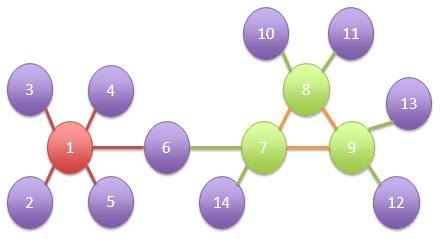
\includegraphics[width=250pt]{../imgs/ej1local.jpg}
\caption{Ejemplo Posible - Usado tambien en Local}
\end{center}
\end{figure}

\textbf{Formato de entrada:}

$$14\ \  14$$
$$1\ \  2$$
$$1\ \  3$$
$$1\ \  4$$
$$1\ \  5$$
$$1\ \  6$$
$$6\ \  7$$
$$7 \ \ 8$$
$$8\ \  9$$
$$9\ \  7$$
$$8\ \  10$$
$$8\ \  11$$
$$9\ \  12$$
$$9\ \  13$$
$$7\ \  14$$


\textbf{Formato de salida:}
$$5\ \   1\ \   1$$

\textbf{solucion optima:}
 $$6\ \   3\ \   7\ \   8\ \   9$$\newline

Se puede observar como a medida que uno agrega adyacentes a los nodos $7$, $8$ o $9$ tal que el nodo de mayor grado sea el $1$ la solucion va a ser tan mala como uno quiera, por ejemplo, agregandole mas adyacentes a $1$, para asi poder aumentar la cantidad de nodos de la frontera de la clique optima. \newline

Notar que la mayoría de problemas encontrados se deben al proceso de intensificación, aunque en muchos casos puede ser muy favorable, en otros seria mejor aplicar técnicas de diversificación, como por ejemplo, variar la entrada por nodos de diferentes cliques máximas, colaborando mucho en la búsqueda de soluciones mas diversas.

\subsection{Experimentación}

 En esta sección buscamos encontrar un numero correcto para asignarle $desviacion\_permitida$ de tal forma de amortiguar lo mas posible tiempo con resultados. \newline
 El siguiente gráfico muestra, para diferentes $desviacion\_permitida$ y una densidad de aristas igual al 50$\%$ respecto a los nodos, el resultado temporal, y luego de calidad. Los grafos son aleatorios, este tipo de grafos son explicitados mas adelante en la sección $Experimentacion\ General$.


\begin{figure}[H] %[h] Aqui [b] para button [t] para top
\begin{center}
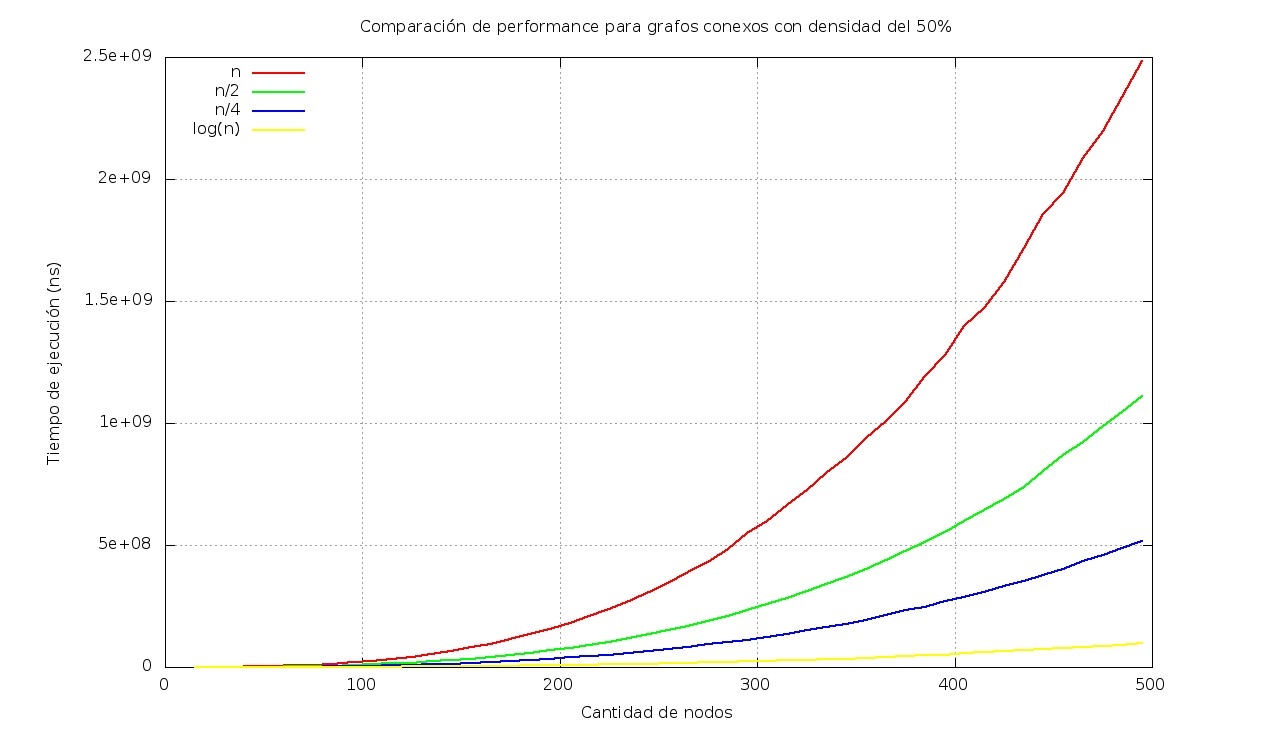
\includegraphics[width=400pt]{../imgs/variaciontemporal_tabu.jpg}
\caption{Variacion de $desviacion\_permitida$ - Grafico Temporal}
\end{center}
\end{figure}

\begin{figure}[H] %[h] Aqui [b] para button [t] para top
\begin{center}
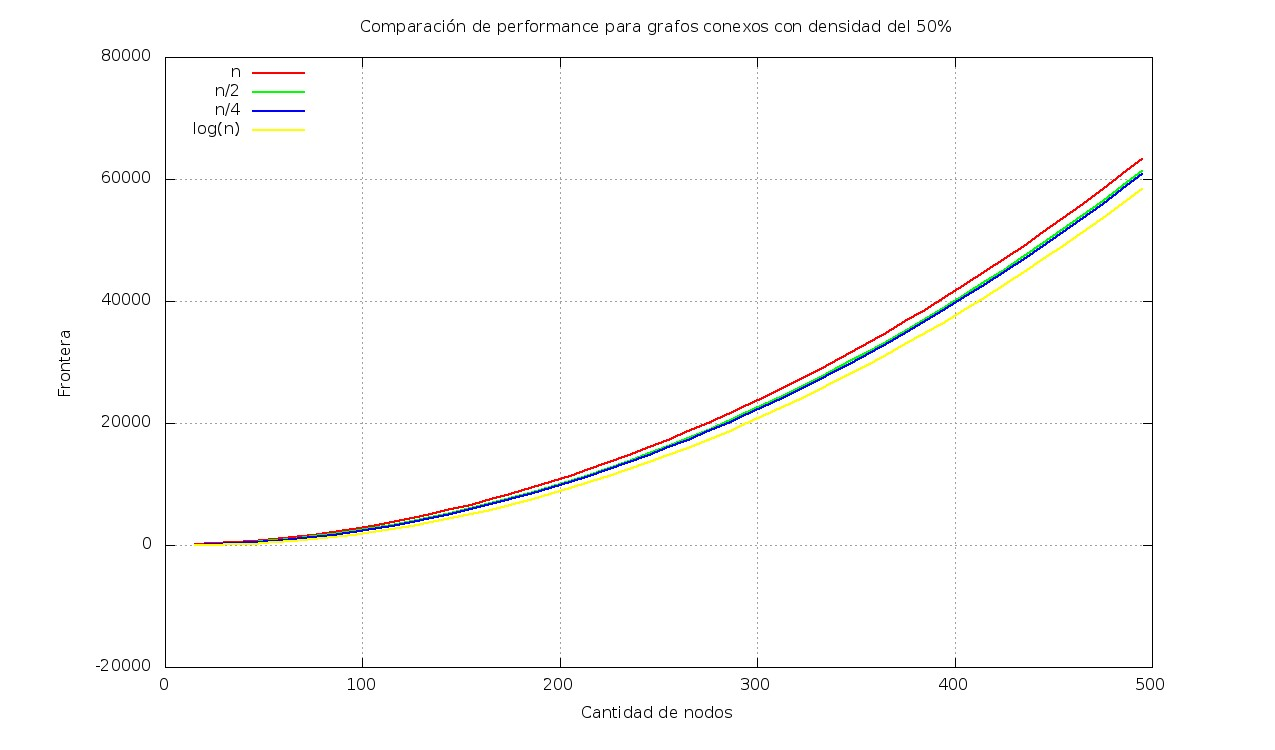
\includegraphics[width=400pt]{../imgs/variacioncalidad_tabu.jpg}
\caption{Variacion de $desviacion\_permitida$ - Grafico de Calidad}
\end{center}
\end{figure}

El siguiente gráfico muestra un promedio entre el tiempo que tarda y el resultado obtenido.

\begin{figure}[H] %[h] Aqui [b] para button [t] para top
\begin{center}
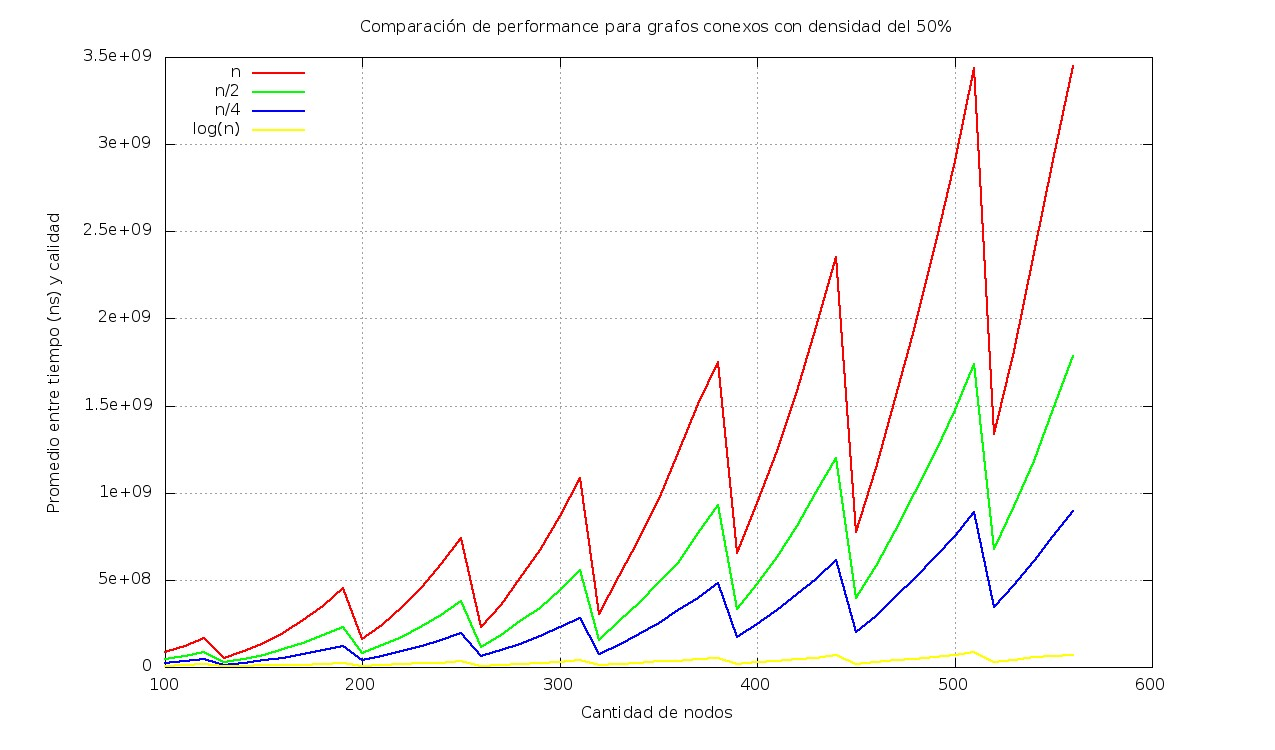
\includegraphics[width=400pt]{../imgs/variacionpromedio_tabu.jpg}
\caption{Variacion de $desviacion\_permitida$ - Grafico Promedio entre calidad y tiempo}
\end{center}
\end{figure}

 Cuando hablamos de promedio hacemos referencia a un balance entre tiempo y calidad. Elegimos esto ya que,  para realizar diferentes experimentaciones con los grafos, dado la densidad y la cantidad de pruebas que hacemos no nos es viable que tarde mucho en procesar cada grafo. A su vez, tampoco queremos que las soluciones nunca mejoren a la local, porque no tendría sentido. Es por esta razón que elegimos el promedio.

 De esta manera podemos observar que para una densidad de 50$\%$ de aristas un valor promedio optimo es $n/2$ con $n$ = $cantidad\ de\ nodos$. Es por esta razón que en los items anteriores usamos este valor. Elegimos este valor, aunque también pudimos haber elegido $n/4$, pero cuanto mas chico, en grafos con pocas aristas va a contemplar muchos menos casos.


\newpage

\section{Experimentación General}
%En el grafico se puede observar como el crecimiento de todos las heuristicas es polinomial a menida que el grafo aumenta su densidad en aristas. A su vez el algoritmo $Tabu$ $Search$ presenta una mayor diferencia en cuanto a tiempo, esto es razonable porque puede empeorar parcialmente la solucion dependiendo la cantidad de nodos, entonces esa diferencia (constante) lo que hace es "subirme" la funcion la cantidad observada. 

Para realizar la experimentación respecto a la calidad de las heurísticas presentadas, utilizamos un generador de las siguientes familias de grafos:
\begin{itemize}
\item Estrella + CMF
 \begin{figure}[H] %[h] Aqui [b] para button [t] para top
\begin{center}
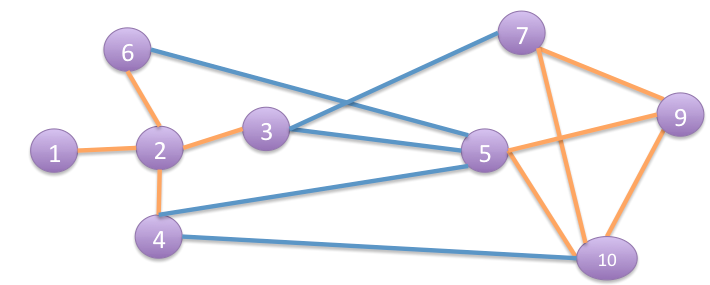
\includegraphics[width=200pt]{../imgs/Estrella+CMF.jpg}
\caption{Grafo de ejemplo de tipo Estrella con una CMF que no esta en la estrella.}
\end{center}
\end{figure}
\item Estrella+Puente+CMF
 \begin{figure}[H] %[h] Aqui [b] para button [t] para top
\begin{center}
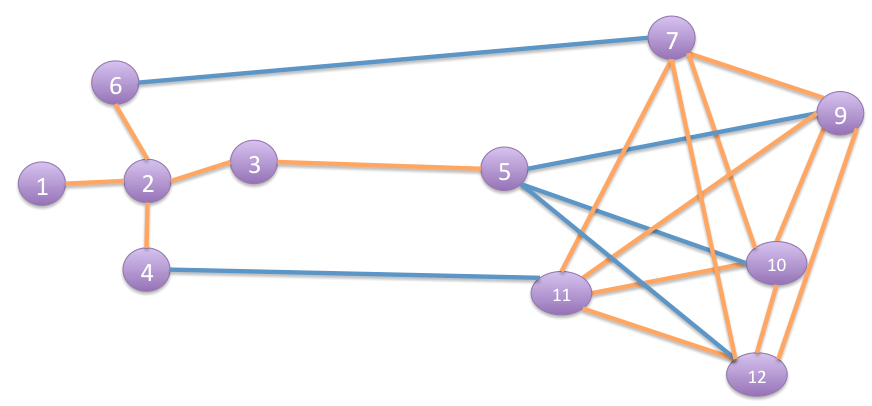
\includegraphics[width=200pt]{../imgs/Estrella+Puente+CMF.jpg}
\caption{Grafo de ejemplo de tipo Estrella con un puente a otra parte del grafo que tiene la CMF}
\end{center}
\end{figure}
\item Estrella+Puente+Doble Estrella
 \begin{figure}[H] %[h] Aqui [b] para button [t] para top
\begin{center}
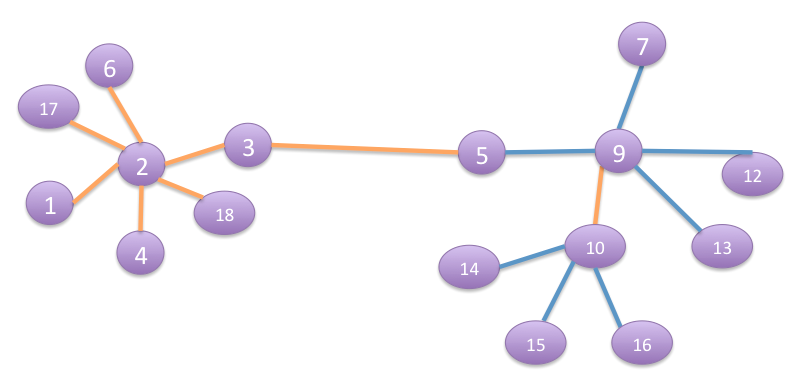
\includegraphics[width=200pt]{../imgs/Estrella+puente+dobleEstrella.jpg}
\caption{Grafo de ejemplo de tipo Estrella con un puente a una estrella doble.}
\end{center}
\end{figure}

\item Banana Tree (Palmera)
 \begin{figure}[H] %[h] Aqui [b] para button [t] para top
\begin{center}
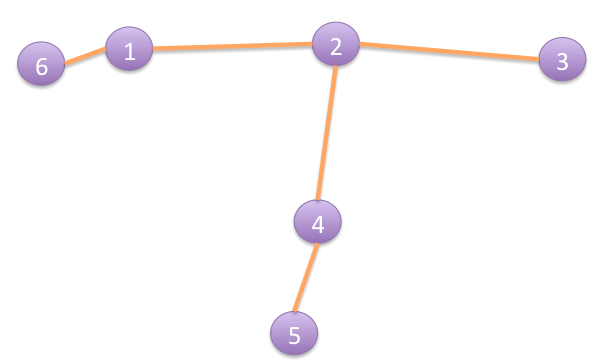
\includegraphics[width=200pt]{../imgs/banana.jpg}
\caption{Grafo de ejemplo de tipo Estrella con un puente a una estrella doble.}
\end{center}
\end{figure}
\item Rueda
 \begin{figure}[H] %[h] Aqui [b] para button [t] para top
\begin{center}
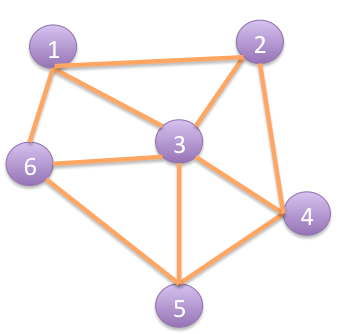
\includegraphics[width=150pt]{../imgs/rueda.jpg}
\caption{Grafo de ejemplo de tipo Estrella con un puente a una estrella doble.}
\end{center}
\end{figure}
\end{itemize}
Luego, procedimos aumentando la cantidad de nodos de los grafos, que a su vez aumenta la cantidad de aristas de éstos dado que los grafos en cuestión se caracterizan por un porcentaje determinado de aristas con respecto a sus nodos. De este modo, realizamos pruebas para cada heurística sobre cada familia de grafos.

Por otro lado, separamos las pruebas de calidad de soluciones en chicas y grandes, esto lo hicimos ya que nos interesa ver la solucion obtenida por el algoritmo exacto para poder compararlo con las heurísticas, y en otro contexto tambien comparar la calidad de las soluciones de las heurísticas para grafos donde el algoritmo exacto no puede resolver a tiempo. 

Las pruebas chicas consisten en grafos de entre 10 y 150 nodos con una densidad de aristas del 50\%. De esta forma, el algoritmo exacto puede encontrar soluciones en un tiempo relativamente rápido y nos permite compararlo con las heurísticas. En el caso de las pruebas grandes, tomamos grafos de entre 200 y 2000 nodos con una densidad de aristas del 50\%. La decisión acerca de la cantidad de aristas se realizó de forma tal a encontrar un balance entre grafos con pocas y muchas aristas, sin afectar demasiado el tiempo de ejecución del algoritmo exacto y de las heurísticas. 


 \begin{figure}[H] %[h] Aqui [b] para button [t] para top
\begin{center}
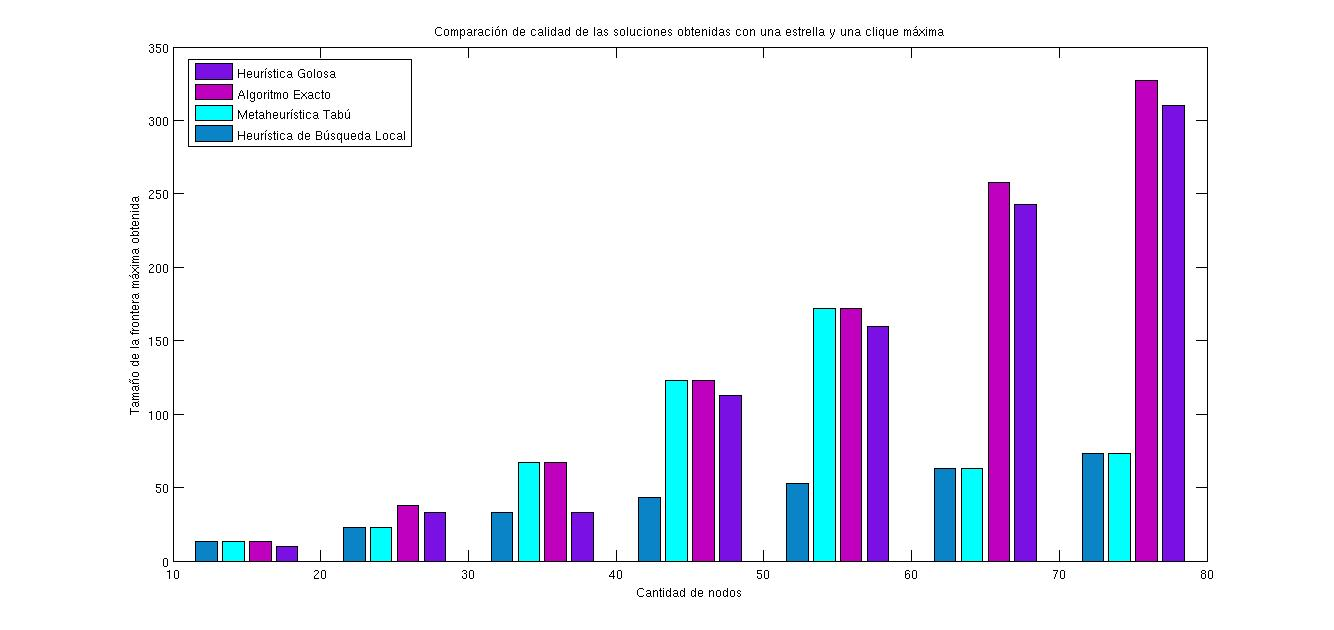
\includegraphics[width=400pt]{../imgs/calidadSolucionesChicas15.jpg}
\caption{Comparación realizada con soluciones chicas con un grafo de tipo Estrella+CMF.}
\end{center}
\end{figure}

En este caso, tenemos una estrella cuyo nodo central no forma parte de la clique de frontera máxima, con lo cual aquellos algoritmos que consideren a los nodos de mayor grado para empezar su ejecución y llegar a un resultado se verán perjudicados por esta familia. Tanto la heurística de búsqueda local como la metaheurística Tabú se ven perjudicadas por la caracterización del grafo, esto se debe a que la heurística parte del nodo de mayor grado y se mueve por una vecindad pequeña y nunca llega a encontrar la CMF que se encuentra a una distancia considerable de la estrella que forma el nodo. En el caso de la metaheurística, lo que sucede es que parte de una solución incial dada por la búsqueda local, con lo cual tiene un punto de partida poco ventajoso que termina provocando que genere un mal resultado. En el caso de la búsqueda golosa, esta se ve beneficiada ya que si bien empieza con el nodo de mayor grado, eventualmente prueba con otros nodos teniendo asá mayor probabilidad de encontrar la clique de frontera máxima. 

 \begin{figure}[H] %[h] Aqui [b] para button [t] para top
\begin{center}
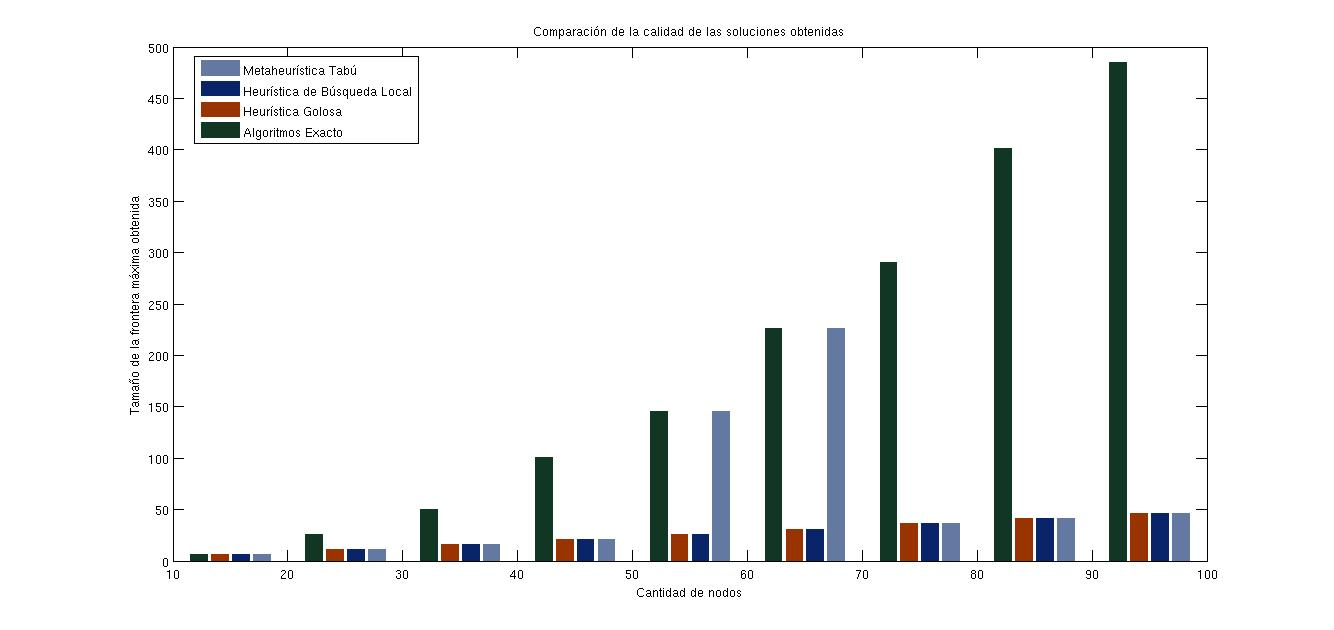
\includegraphics[width=400pt]{../imgs/calidadSolucionesChica14.jpg}
\caption{Comparación realizada con soluciones chicas con un grafo de tipo Estrella+Puente+CMF.}
\end{center}
\end{figure}



En este caso sucede lo mismo que en el anterior, los algoritmos inician en la estrella ya que ésta tiene mayor grado y provoca que nunca se logren mover hasta las soluciones que se encuentran del otro lado del puente que se forma entre la estrella y la estructura que contiene una clique de frontera máxima del otro lado.

 \begin{figure}[H] %[h] Aqui [b] para button [t] para top
\begin{center}
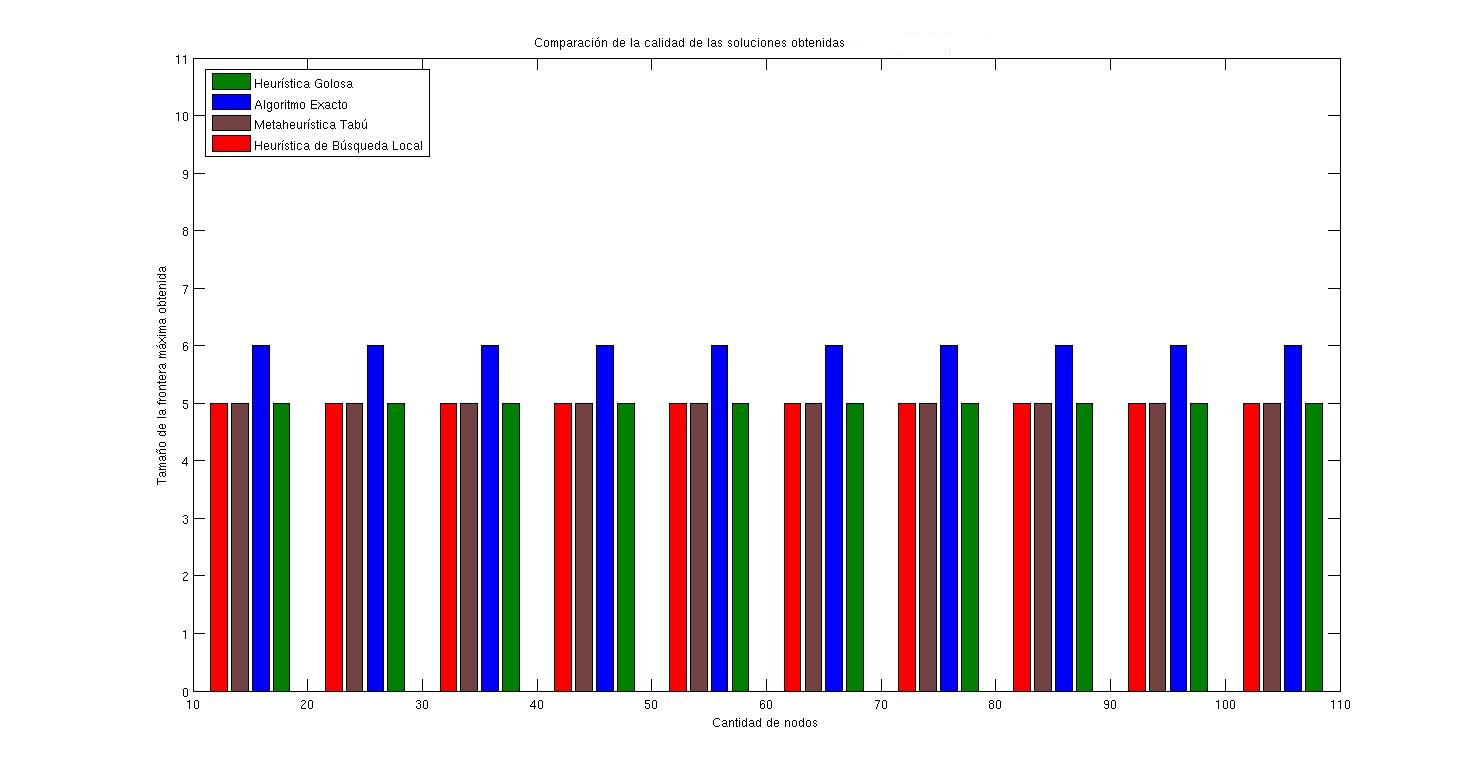
\includegraphics[width=400pt]{../imgs/calidadSolucionesChicas17.jpg}
\caption{Comparación realizada con soluciones chicas con un grafo de tipo Estrella+Puente+Doble Estrella.}
\end{center}
\end{figure}


En este caso, el grafo se caracteriza por contener una estrella que está conectada con dos estrellas. Estas dos estrellas forman una clique de frontera maxima que no contiene al nodo de la primera estrella. Lo que sucede es que la solución de la estrella es parecida a la solucion correcta del problema, pero esta no es la mejor que encuentra el exacto, por eso las heurísticas se quedan con ella mientras que el exacto encuentra la mejor solución entre las estrellas que estan unidas.


 \begin{figure}[H] %[h] Aqui [b] para button [t] para top
\begin{center}
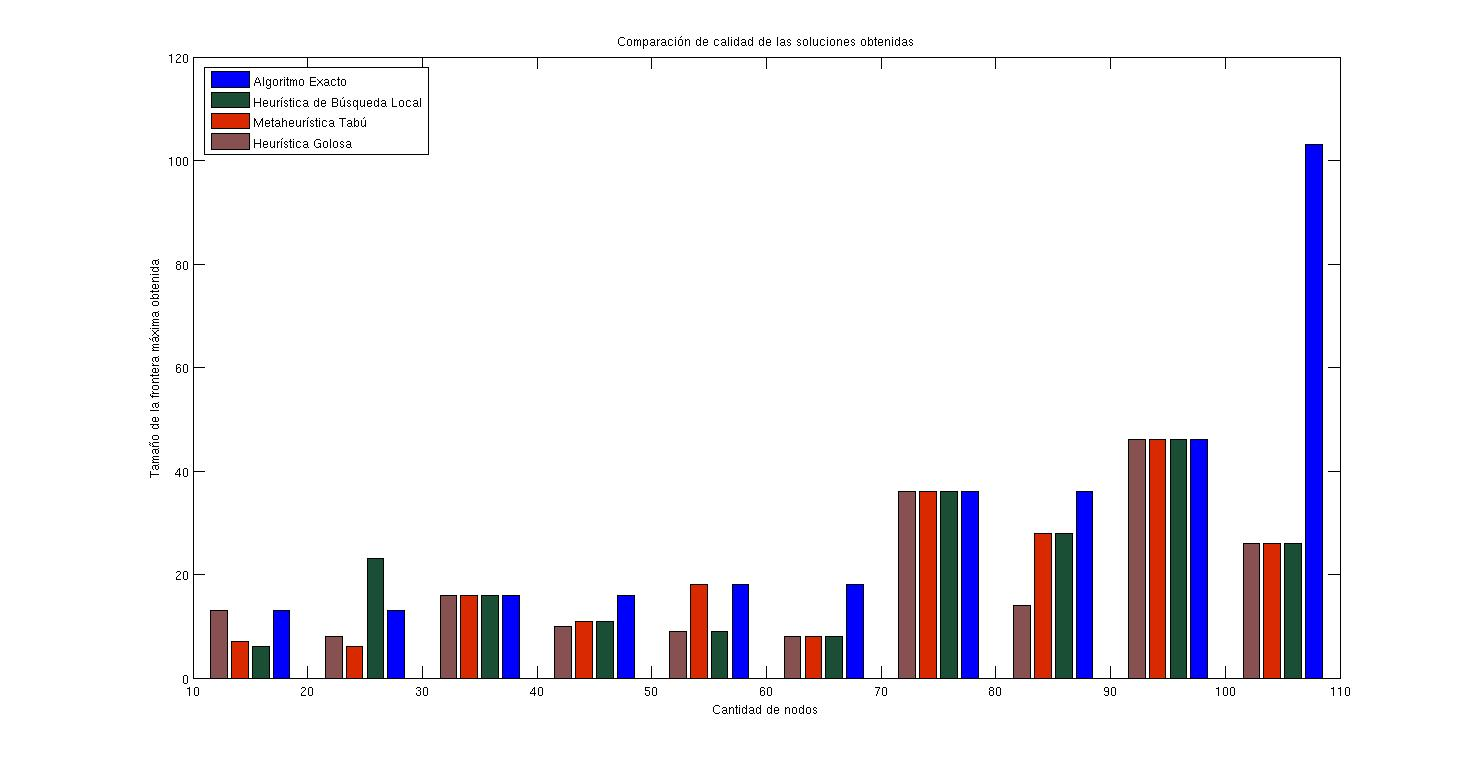
\includegraphics[width=400pt]{../imgs/calidadSolucionesChicas3.jpg}
\caption{Comparación realizada con soluciones chicas con un grafo de tipo Banana Tree.}
\end{center}
\end{figure}

En este caso, tenemos un grafo de tipo banana tree, las heurísticas en la mayoría de los casos obtuvieron soluciones correctas.

 \begin{figure}[H] %[h] Aqui [b] para button [t] para top
\begin{center}
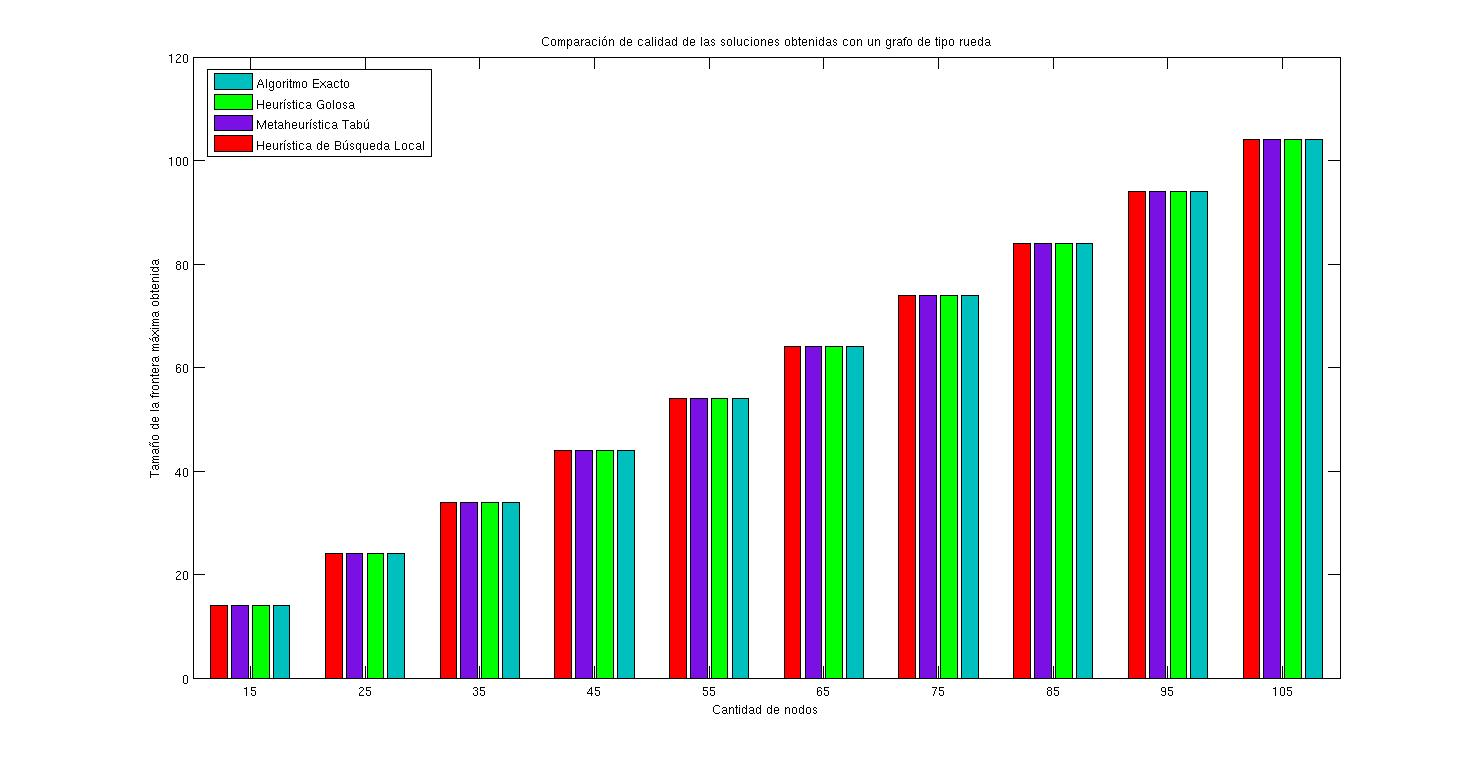
\includegraphics[width=400pt]{../imgs/calidadSolucionesChicas2.jpg}
\caption{Comparación realizada con soluciones chicas con un grafo de tipo rueda.}
\end{center}
\end{figure}

 \begin{figure}[H] %[h] Aqui [b] para button [t] para top
\begin{center}
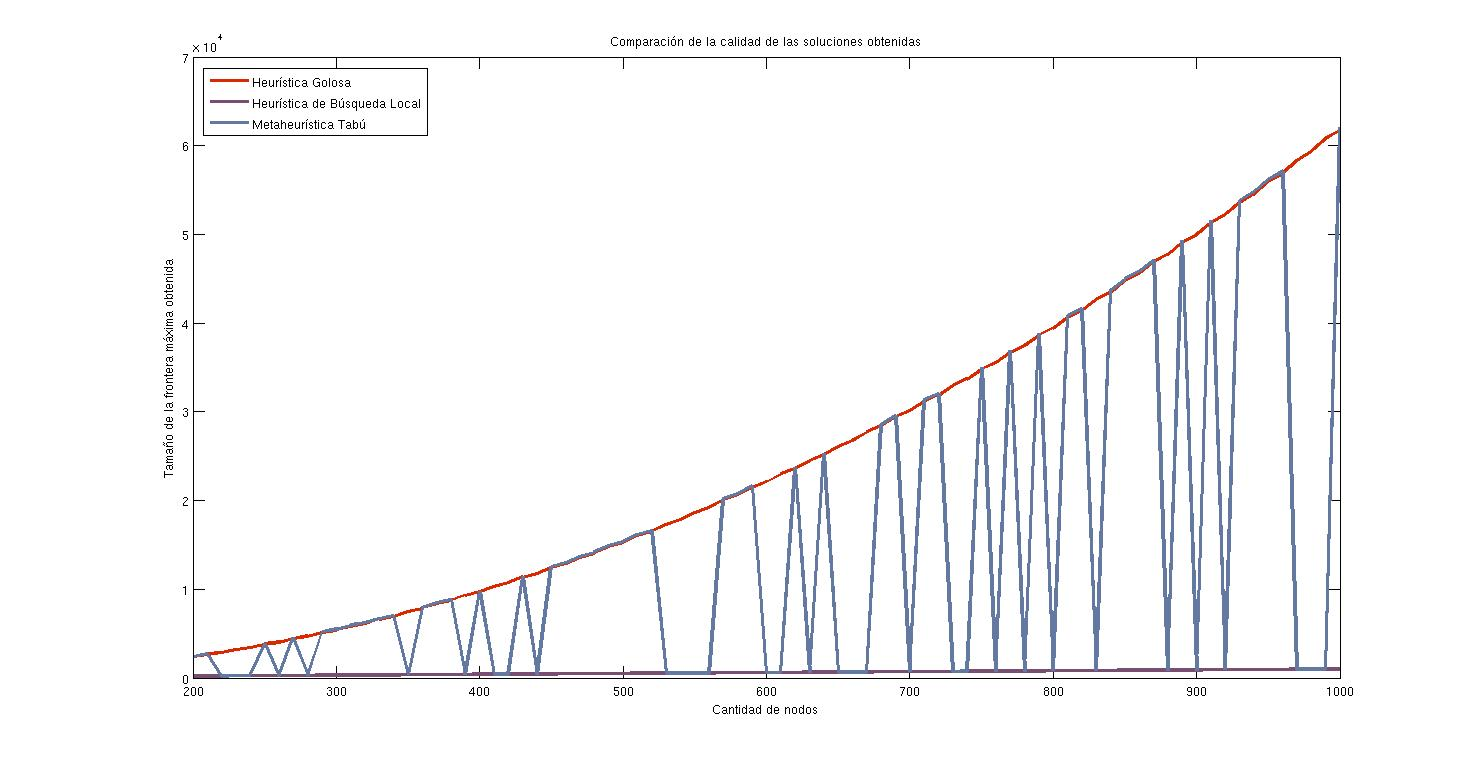
\includegraphics[width=400pt]{../imgs/calidadSolucionesGrandes15.jpg}
\caption{Comparación realizada con soluciones grandes con un grafo de tipo Estrella+CMF.}
\end{center}
\end{figure}

 \begin{figure}[H] %[h] Aqui [b] para button [t] para top
\begin{center}
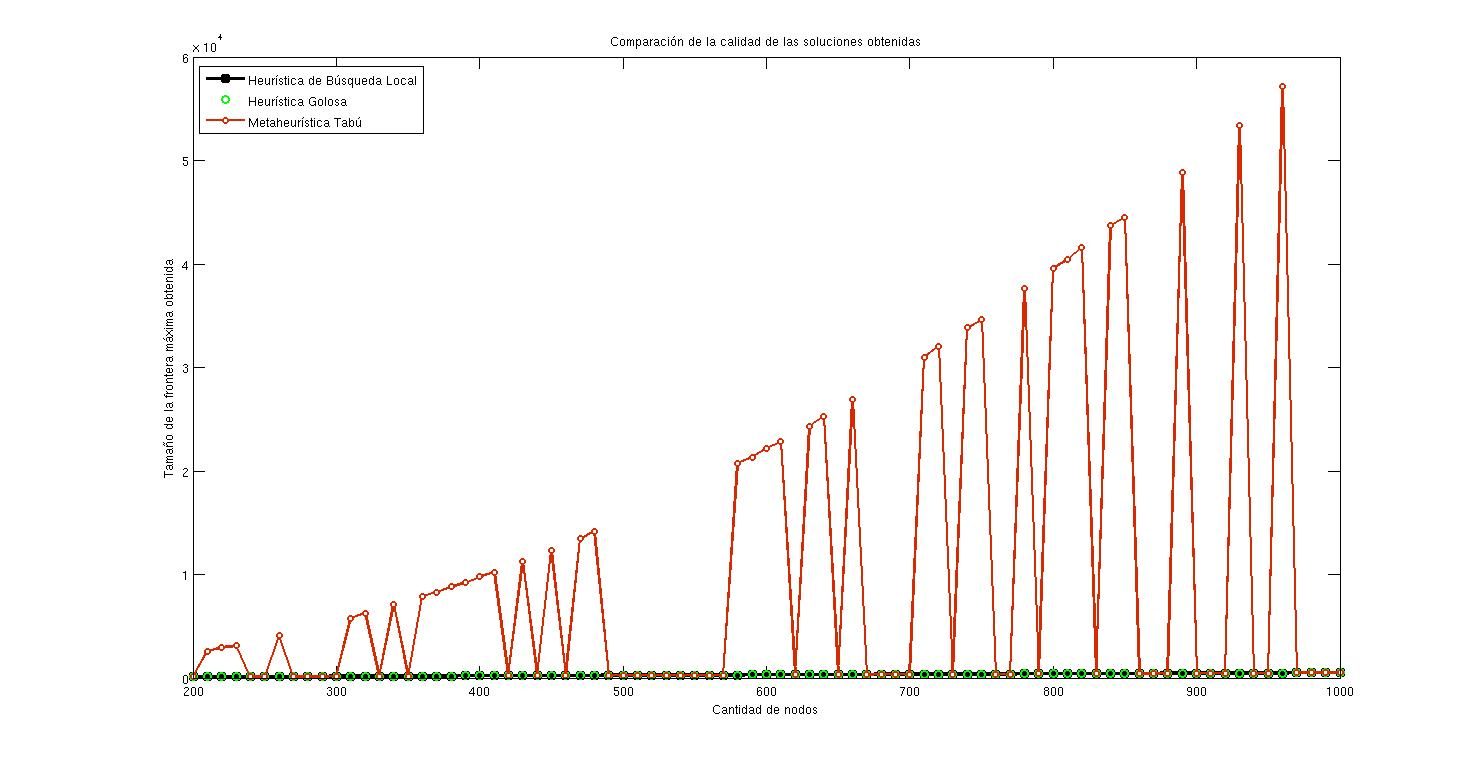
\includegraphics[width=400pt]{../imgs/calidadSolucionesGrandes14.jpg}
\caption{Comparación realizada con soluciones grandes con un grafo de tipo Estrella+Puente+CMF.}
\end{center}
\end{figure}

 \begin{figure}[H] %[h] Aqui [b] para button [t] para top
\begin{center}
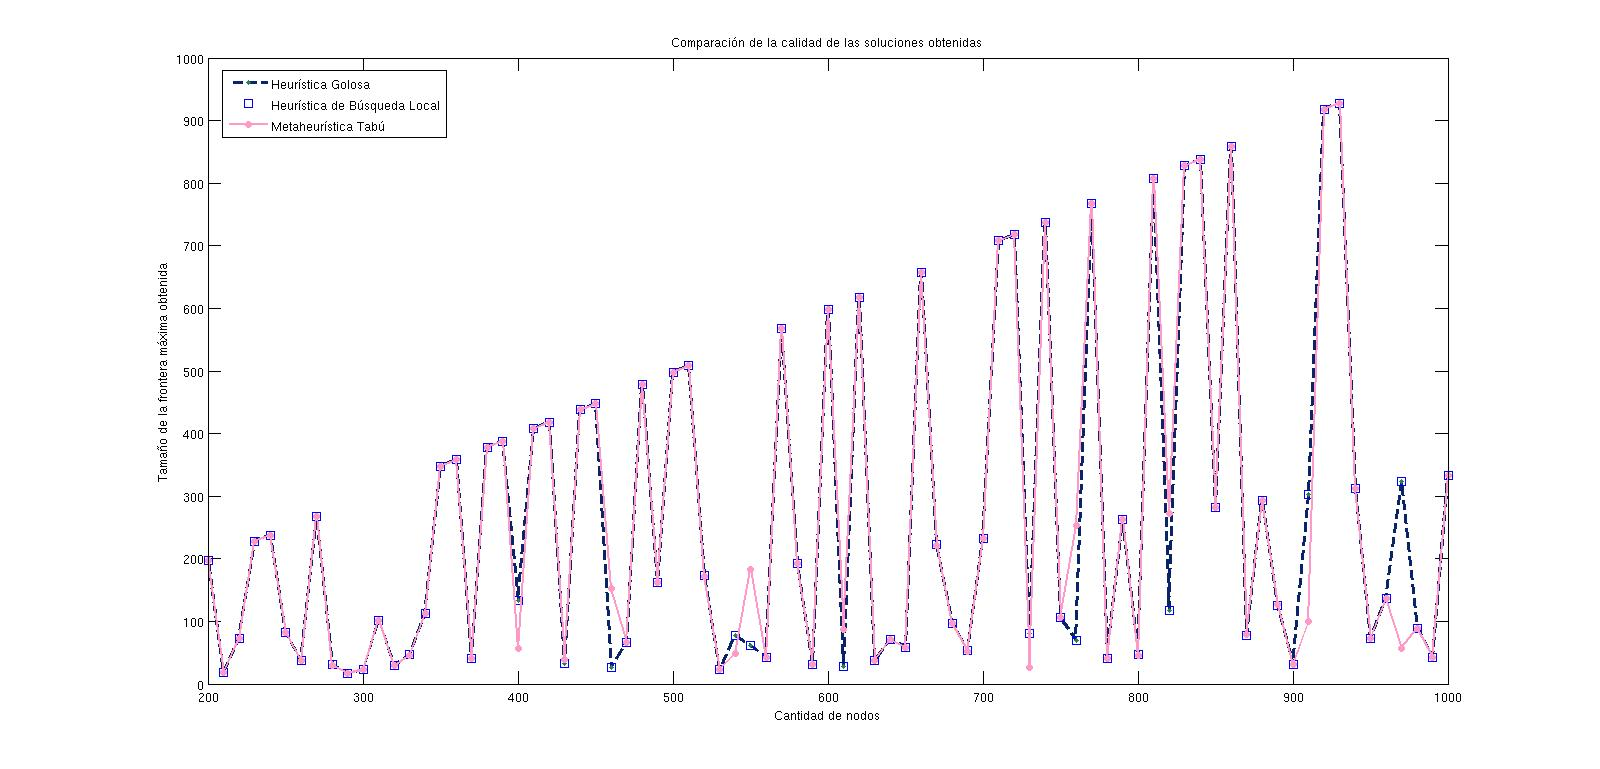
\includegraphics[width=400pt]{../imgs/calidadSolucionesGrandes3.jpg}
\caption{Comparación realizada con soluciones grandes con un grafo de tipo Banana Tree.}
\end{center}
\end{figure}







\newpage

\section{Referencias}
\begin{itemize}
\item CORMEN, THOMAS H. ; Introduction to Algorithms, Third ed. 2009. The MIT Press.
\end{itemize}


\section{Código fuente}


\end{document}
